% 1. PAPclass muss geladen werden, der Dateipfad wird angegeben. Problem ist, dass \documentclass{} keine Dateipfade verarbeiten kann
\makeatletter
\def\input@path{{../latex_class/}} % Relativer Pfad zum Ordner mit der .cls
\makeatother
% man könnte alternativ auch die PAPclass.cls in das lokale TeX-Verzeichnis der Installation legen, dann würde die Datei immer gefunden werden

% use [draft] for quicker compiling (only loads images as frames and enables showkeys - labels are shown)
\documentclass[final,ngerman]{PAPclass}   % to select the document's language, I tested multiple options and the best one is to use it as a global option so its passed down to all packages in PAPclass (especially to cleverref). One could use no main-language option and load \usepackage[english,ngermn]{babel} so ngerman as the second loaded language is automatically selected as default and then \selectlanguage{english} if needed. But without using \usepackage[ngerman]{cleverref}, the reference-abbreviations (e.g. fig 1.2) are still in english. So one must pass the global option to cleverref or set it locally - and locally is not that fun. All variable settings should be accessable in the main.tex. If you stick with babel loading options and set ngerman as a global option, then babel prints an error.
\input{../latex_class/cmds.tex}

% %comment% these in case of an english document
\captionsetup[figure]{name=Abb.}
\captionsetup[wrapfigure]{name=Abb.}

% Grafikpfade festlegen
\graphicspath{{./images/}{../Diagramme/}{../Bilder/}}
% \svgpath{{../../Messwerte/}} % if you can bring your tex installation to compile svgs - congrats, pls send me an email: b.k.ballcr@gmail.com and tell me how its done

%pages= {1-27},
% Biblatex Einstellungen vornehmen
\addbibresource{../latex_class/lit.bib}                         % initialisieren der .bib Datei
\defbibfilter{literature}{not keyword=figure}
\defbibfilter{figures}{keyword=figure}
% \NewBibliograhpyString{ZuletztOnline}                            % some way probably to automate setting a date, but idk
% \DefineBibliographyStrings{german}{ZuletztOnline = {[Online, Stand 02/2026]}}

% KOMA-Script Einstellungen für Header und footer
\clearpairofpagestyles
\setkomafont{pageheadfoot}{\footnotesize}
\setkomafont{pagehead}{\scshape}
\setkomafont{pagination}{}
\ihead{\versuchnummer\;- \versuch}
\ohead{\headmark}
\cfoot{\pagemark}


%-Document settings
% -- Variable Settings
\newcommand{\documentTitle}{Auswertung Versuch }	    % Titel
\newcommand{\versuchnummer}{01}
\newcommand{\versuch}{Grundpraktikum Elektronik}
\newcommand{\tutor}{Penelope Hoffmann}               % Tutor:in
\newcommand{\Termin}{17.-19.08.2026}	

% -- Fixed Settings
\newcommand{\documentAuthor}{Benjamin Kleijn, Patrick Gottwald}       % Autor				
% \newcommand{\Abschluss}{Bachelor of Science}	
\newcommand{\department}{Physik}	                % Fachrichtung
\newcommand{\locationUniversity}{Heidelberg}	    % Uni Standort
% \newcommand{\Gruppe}{9}	                        % Gruppe
\newcommand{\Kurs}{nachmittags}


%% ------------------------------
%% |    Versuchsausarbeitung    |
%% ------------------------------
\begin{document}
    \begin{titlepage}
\begin{figure}[t]
	\centering
	\textbf{\textsf{\Large we're in awe}}\\\vspace{0.3cm}
	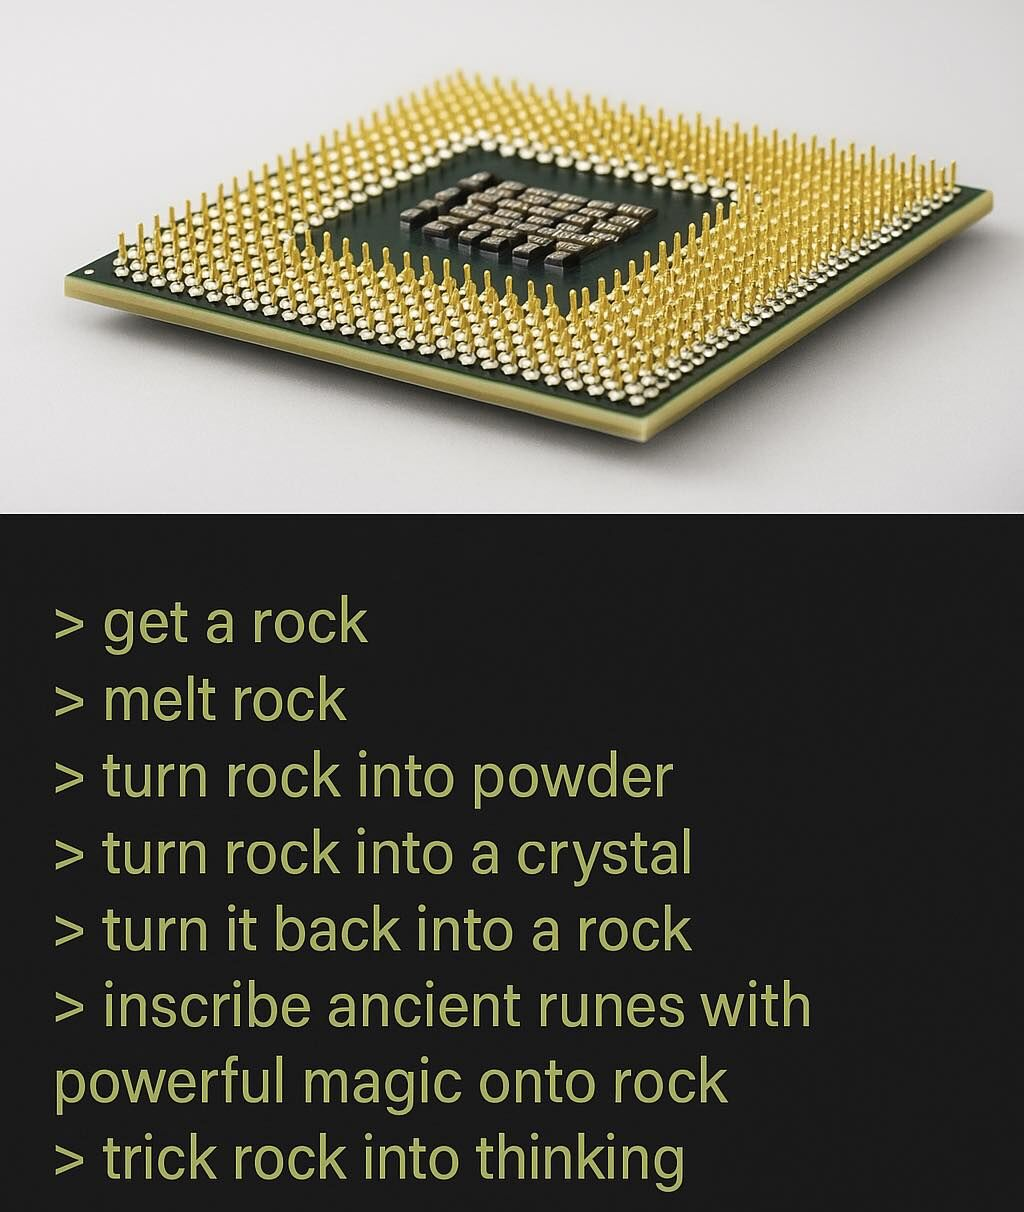
\includegraphics[width=9cm]{magicrocks.png}
	\caption[\emph{Meme:} Magic rocks created by powerful magic\autocite{magicrocks}]{Memes about magic rocks written with magic rocks, shared with magic rocks, presented by magic rocks\autocite{magicrocks}}
\end{figure}

\begin{center}

\enlargethispage{20mm}
	\vspace*{4mm}	{\LARGE\textbf \documentTitle \LARGE\textbf \versuchnummer\;- \versuch}\\
    \vspace*{6mm}	{\large\textbf {Fortgeschrittenen Praktikum FP}}\\
	
	\vspace*{6mm}  {des Studienganges \department}\\
	\vspace*{3mm}  {an der Universität \locationUniversity} \\

	\vspace*{6mm}  {von}\\
	\vspace*{3mm}  {\large\textbf{\documentAuthor}}\\
	\vspace*{12mm}  {\today}\\

\vfill

{	
\begin{tabular}{@{}rl@{}}
	\textbf{Versuchstermin} & \Termin \\
	% \textbf{Gruppe} & \Gruppe \\
	\textbf{Tutor:in}		& \tutor\\
  \end{tabular}
}
\end{center}

\end{titlepage}

    \clearpage
    \pagestyle{scrheadings}

    \tableofcontents
    \clearpage
    \listoffigures
    \listoftables
    \clearpage                    
    \section{Einleitung}                                % Die Texte werden in den einzelnen Dateien eingefügt.
    Das Auseinandersetzen mit Transistoren ist unabdingbar, um ein Gefühl für die Hintergründe und Funktionsweisen der technischen Bauteile zu bekommen, deren Verfeinerung, Verbesserung und Weiterentwicklung die Digitale Revolution in einer Dimension ermöglicht, die alle Bereiche der menschlichen Zivilisation von Grund auf verändert. 

Zudem sind Löt- und Grundlagenkenntnisse elektrischer Schaltungen ein wesentlicher Bestandteil der Realisation von Experimenten und eigenen Anwendungen, das Beschäftigen mit diesen Bereichen ist also von großer Bedeutung für Physiker:innen (und natürlich auch von Interesse für von Elektronik faszinierte Menschen). Außerdem wurde weiter Erfahrung im Umgang mit Oszilloskopen gesammelt, was auch ein wichtiger Skill für Physiker:innen ist.

Final liegt der Charme dieses Versuches in dem sukzessiven Verstehen der Bestandteile und Aufbauen eines hochgradig fähigen Systems, dem PID-Regler, dessen Schaltplan \cite[vgl.][11]{Skript_01} zwar auf den ersten Blick überwältigend aussieht, auf den zweiten Blick jedoch nur aus geschickter Kombination bekannter Bauteilen besteht. Ein PID-Regler basiert auf der eleganten Nutzung von Operationsverstärkern, deren Innenleben zwar nur aus Widerständen, Kondensatoren und Transistoren besteht, jedoch alles andere als trivial ist:
\xfigure{htbp}{width=0.8\textwidth}{OpAmpTransistor.png}{\emph{Meme:} Which part don't you understand?\autocite{OpAmpTransistorLevelColored}}{ist der Operationsverstärker wirklich bekannt? \autocite{OpAmpTransistorLevelColored}}

\paragraph{PID-Grundlagen:} Es gibt gute Youtube-Videos über PID-Controlling: kurzer Überblick: \href{https://youtu.be/wkfEZmsQqiA?si=atU3_SOSYyGcCa4w}{\emph{What Is PID Control?}} mit Beispiel und hier ein etwas komplexeres Beispiel \href{https://www.youtube.com/watch?v=XfAt6hNV8XM}{\emph{Simple Examples of PID Control}}, das die Eigenschaften von P-, I-, D-, PID-Controllern aufzeigt.
    \clearpage
    \section{Durchführung}
    Emitterwiderstände haben nicht die korrekte Anzahl an stellen.
\todo{Patrick Protokoll anpassen}
Fehlerformel für Widerstände aufschreiben. 
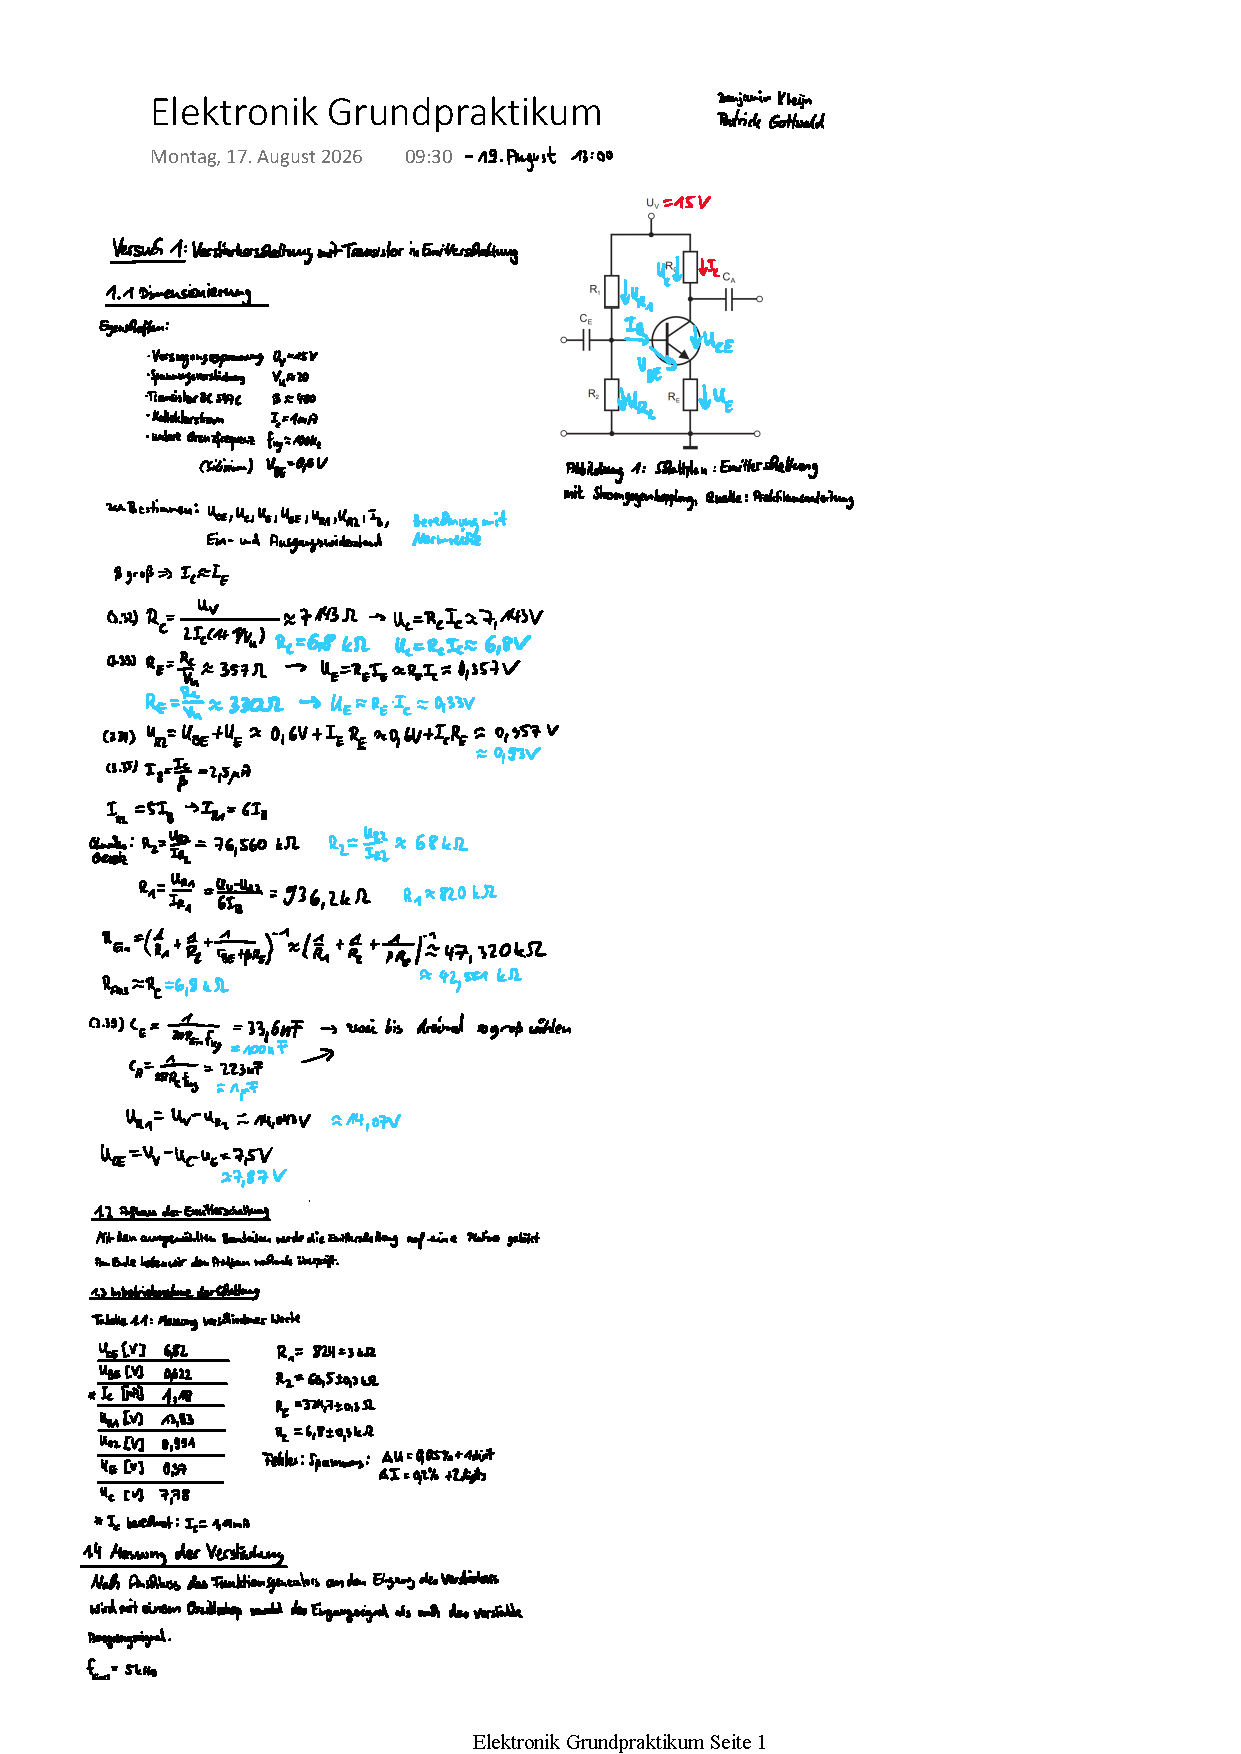
\includepdf[pages=1-7, addtotoc={1, subsection, 2, Messprotokoll, Messprotokoll}]{../../Elektronik Grundpraktikum.pdf}
% % Eigene S-Spalte mit festem Zahlenformat
% \newcolumntype{N}{S[table-format=3.2]}

% \begin{table}[htb]
%   \centering
%   \caption{Dimensionierung der Emitterschaltung}
%   % N ist die Zahl, @{\,} setzt einen kleinen Abstand, l ist die Einheit
%   \begin{tabularx}{0.8\textwidth}{X N @{\,} l N @{\,} l}
%     \toprule
%     Bauteil & \multicolumn{2}{c}{theoretisch} & \multicolumn{2}{c}{Normreihe} \\
%     \midrule
%     $R_C$            &   7.14 & \unit{\kilo\ohm} &   6.80 & \unit{\kilo\ohm} \\
%     $R_E$            & 357.14 & \unit{\ohm}      & 330.00 & \unit{\ohm} \\
%     $R_1$            & 936.19 & \unit{\kilo\ohm} & 820.00 & \unit{\kilo\ohm} \\
%     $R_2$            &  76.57 & \unit{\kilo\ohm} &  68.00 & \unit{\kilo\ohm} \\
%     $C_{\text{EIN}}$ &  33.63 & \unit{\nano\farad}& 100.00 & \unit{\nano\farad} \\
%     $C_{\text{AUS}}$ & 222.82 & \unit{\nano\farad}&   1.00 & \unit{\micro\farad} \\
%     \bottomrule
%   \end{tabularx}
%   \label{table:emitterschaltung}  
% \end{table}

    \clearpage
    \section{Auswertung}\label{sec:Auswertung}
    \subsection*{Formeln der statistischen Analyse\autocite{Skript_01}}
    \input{../latex_class/Statistik.tex}
    \renewcommand{\thesubsection}{\thesection.\Roman{subsection}}

\subsection{Messungen an der Emitterschaltung}
\begin{table}[htbp]
\centering
\caption{Vergleich der experimentellen und berechneten Messwerte an der Emitterschaltung}
\begin{tabularx}{\textwidth}{LZZZZS[table-format =2.1]}
    \toprule
         \text{Messreihe} & x_{\text{exp.}}& x_{\text{calc.}} & \text{abs. Abw.} & \text{proz. Abw.}[\unit{\percent}] & {\(S[\sigma]\)} \\\midrule
       R_C\;[\unit{\kilo\ohm}] & \num{6.810(15)} & 6.8 & \num{0.010(15)} & \num{0.15(0.22)} & 0.7 \\
       R_E\;[\unit{\ohm}] & \num{324.7(0.8)} & 330.0 & \num{5.3(0.8)} & \num{1.63(0.24)} & 8.0 \\
       R_1\;[\unit{\kilo\ohm}] & \num{824.0(18)} & 820.0 & \num{4.0(18)} & \num{0.49(0.22)} & 2.3 \\
       R_2\;[\unit{\kilo\ohm}] & \num{66.50(15)} & 68.0 & \num{1.50(15)} & \num{2.26(0.22)} & 11.0 \\
       \midrule
       U_{\text{CE}}\;[\unit{\volt}] & \num{6.820(0.014)} & 7.87 & \num{1.050(0.014)} & \num{15.40(0.20)} & 80.0 \\
       U_{\text{BE}}\;[\unit{\volt}] & \num{0.6220(0.0014)} & 0.6 & \num{0.0220(0.0014)} & \num{3.54(0.22)} & 17.0 \\
       U_{\text{C}}\;[\unit{\volt}] & \num{7.780(0.014)} & 6.8 & \num{0.980(0.014)} & \num{12.60(0.18)} & 80.0 \\
       I_{\text{C}}\;[\unit{\milli\ampere}] & \num{1.40(21)} & 1 & \num{0.40(21)} & \num{29(16)} & 2.0 \\
       U_{\text{E}}\;[\unit{\volt}] & \num{0.370(0.011)} & 0.33 & \num{0.040(0.011)} & \num{11(3)} & 4.0 \\
       U_{R_1}\;[\unit{\volt}] & \num{13.930(0.017)} & 14.07 & \num{0.140(0.017)} & \num{1.01(0.13)} & 9.0 \\
       U_{R_2}\;[\unit{\volt}] & \num{0.9910(0.0015)} & 0.93 & \num{0.0610(0.0015)} & \num{6.16(0.16)} & 50.0 \\
\bottomrule
\end{tabularx}
\label{table:Vergleich_emitter} 
\end{table}
Offensichtlicherweise basieren die berechneten Werte auf Annahmen, die nur ungefähr getroffen wurden: \(\beta=400\) und \(U_{\text{BE}}=\qty{0.6}{\volt}\) aus der Berechnung entsprechen nicht den realen Werten aus dem Datasheet. Es gibt für diese beiden Werte keine exakten Angaben (\(U_{\text{CE}}\) und \(I_C\) abhängig, temperaturabhängig), die absolute Abweichung zwischen gewollter und experimentell vorliegender Kapazität ist auch unbekannt. Dadurch können die berechneten Werte gar nicht exakt dem untersuchten System entsprechen, was eine größere absolute Abweichung zwischen calc und exp Werten zur Folge hat. Diese Abweichung ist jedoch in der Interpreation der Sigma-Abweichungen zu vernachlässigen, denn die absoluten Abweichungen sind stets gering, die Größenordnung der berechneten Werte ist natürlich richtig. Der weitaus dominierende Grund für die hohen Sigma-Abweichungen ist der winzige Fehler, der sich bisher nur aus dem Messfehler des Multimeters zusammensetzt. Faktoren wie Temperatur,  

\paragraph{Frequenzgang}
Die gemessenen Werte des Frequenzgangs aus Tabelle 1.2 des \href{Messprotokoll}{Messprotokolls} werden nun in ein doppelt-logarithmisches Diagramm aufgetragen. Anschließend wird eine Funktion der Form
\begin{equation}
  f (V, f, W_1, W_2, n_1, n_2) = \frac{V}{\sqrt{1 + \left(\frac{f}{W_1}\right)^{2n_1}} \sqrt{1 + \left(\frac{f}{W_2}\right)^{2n_2}}}
\end{equation}
über die Messwerte gefittet. Aus dem Fit kann schließlich die untere Grenzfrequenz $f_\text{ug}$ bestimmt werden.

\xfigure{htbp}{width=0.8\textwidth}{Frequenzgang_Fit_Emitterschaltung.png}{Frequenzgang der Emitterschaltung mit Fit und eingezeichneter Grenzfrequenz}{Frequenzgang der Emitterschaltung mit Fit und eingezeichneter Grenzfrequenz}
Aus dem Diagramm erhalten wir die Grenzfrequenz $\boxed{f_\text{ug}=31.2 \, \text{Hz}}$.

\subsubsection{Gleichstromgegenkopplung}
siehe \href{Messprotokoll}{Messprotokoll}.

\subsection{Kollektorschaltung}




\paragraph{Frequenzgang}
Nun werden die Messwerte des Frequenzgangs der Kollektorschaltung aus Tabelle 2.2 des \href{Messprotokoll}{Messprotokolls} geplottet. Für die Fitfunktion wird ein Zusammenhang der Form
\begin{equation}
  g (V, f, W_1, n_1) = \frac{V}{\sqrt{1 + \left( \frac{W_1}{f} \right)^{2 \cdot n_1}}}
\end{equation}
verwendet. Schließlich kann man wieder die untere Grenzfrequenz $f_\text{ug}$ aus dem Fit bestimmen, indem untersucht, wann der Fit auf das $\frac{1}{\sqrt{2}}$-Fache gesunken ist.
\xfigure{htbp}{width=0.8\textwidth}{Frequenzgang_Fit_Kollektorschaltung.png}{Frequenzgang der Kollektorschaltung mit Fit und eingezeichneter Grenzfrequenz}{Frequenzgang der Kollektorschaltung mit Fit und eingezeichneter Grenzfrequenz}

Für die Grenzfrequenz ergibt sich somit $\boxed{f_\text{ug}=30.5 \, \text{Hz}}$.

\subsection{Bestimmung der Länge des Koaxialkabels}
Aus dem Protokoll entnehmen wir die berechnete Länge des verwendeten Kabels $l=\qty{13.54(28)}{\meter}$. Der angegebene Wert ist $l_\text{ang}= \qty{13.5}{\meter}$. Die Abweichung beträgt somit $S=0.14 \sigma$.
% \begin{table}[htb]
%   \centering
%   \caption{}
%   \begin{tabularx}{\textwidth}{ZZZZ}
%     \toprule
%             \cmidrule[0.3pt](l{1.0cm}r{1.5cm}){1-4}
%     \bottomrule
%   \end{tabularx}
% \label{table:}  
% \end{table}
    \newpage
    \section{Diskussion}
    \subsection{Emitterschaltung}





\subsection{Kollektorschaltung}
\paragraph{Länge des Koaxialkabels}
Die bestimmte Länge und angegebene Länge haben mit $S=0.14\sigma$ eine sehr geringe Abweichung. Jedoch sei hier angemerkt, dass die Abschätzung der Signalgeschwindigkeit auf 2/3 der Lichtgeschwindigkeit recht ungenau ist, in der Berechnung aber als perfekt angenommen wurde.

\paragraph{Impedanz des Koaxialkabels} Im Versuch wurde die Impedanz des verwendeten Koaxialkabels zu $R=54.60(21)$ bestimmt. Dies entspricht den typischen Werte für Koaxialkabel, die laut Wikipedia \autocite{Koaxialkabel} bei \(50-75 \, \Omega\) liegen.


\subsection{PID-Regler}

\subsubsection{Interner Sollwert} Die Anpassung des Motors an den eingestellten Sollwert erfolgt, wie erwartet, schneller, wenn die P-Regelung aktiviert ist. Wenn sie deaktiviert ist, dann passiert die  Anpassung etwas verzögert, aber trotzdem recht schnell.
Wenn man nun zusätzlich noch I- und D-Anteil hinzuschaltet, wird die Regelung weiter optimiert.

\subsubsection{Externer Sollwert}

Nun steuert ein Funktionsgenerator den Sollwert über ein eingestelltes Rechteck-Signal. Dabei werden nun die Regelungen getrennt für die P-Regelung, die PI-Regelung und für die PD-Regelung untersucht und schließlich mit der PID-Regelung optimiert.
\paragraph{P-Regelung}
Hier ist der I- und der P-Anteil ausgeschaltet.
\begin{figure}[htbp]
    \begin{subfigure}[b]{0.48\textwidth}
    \centering
    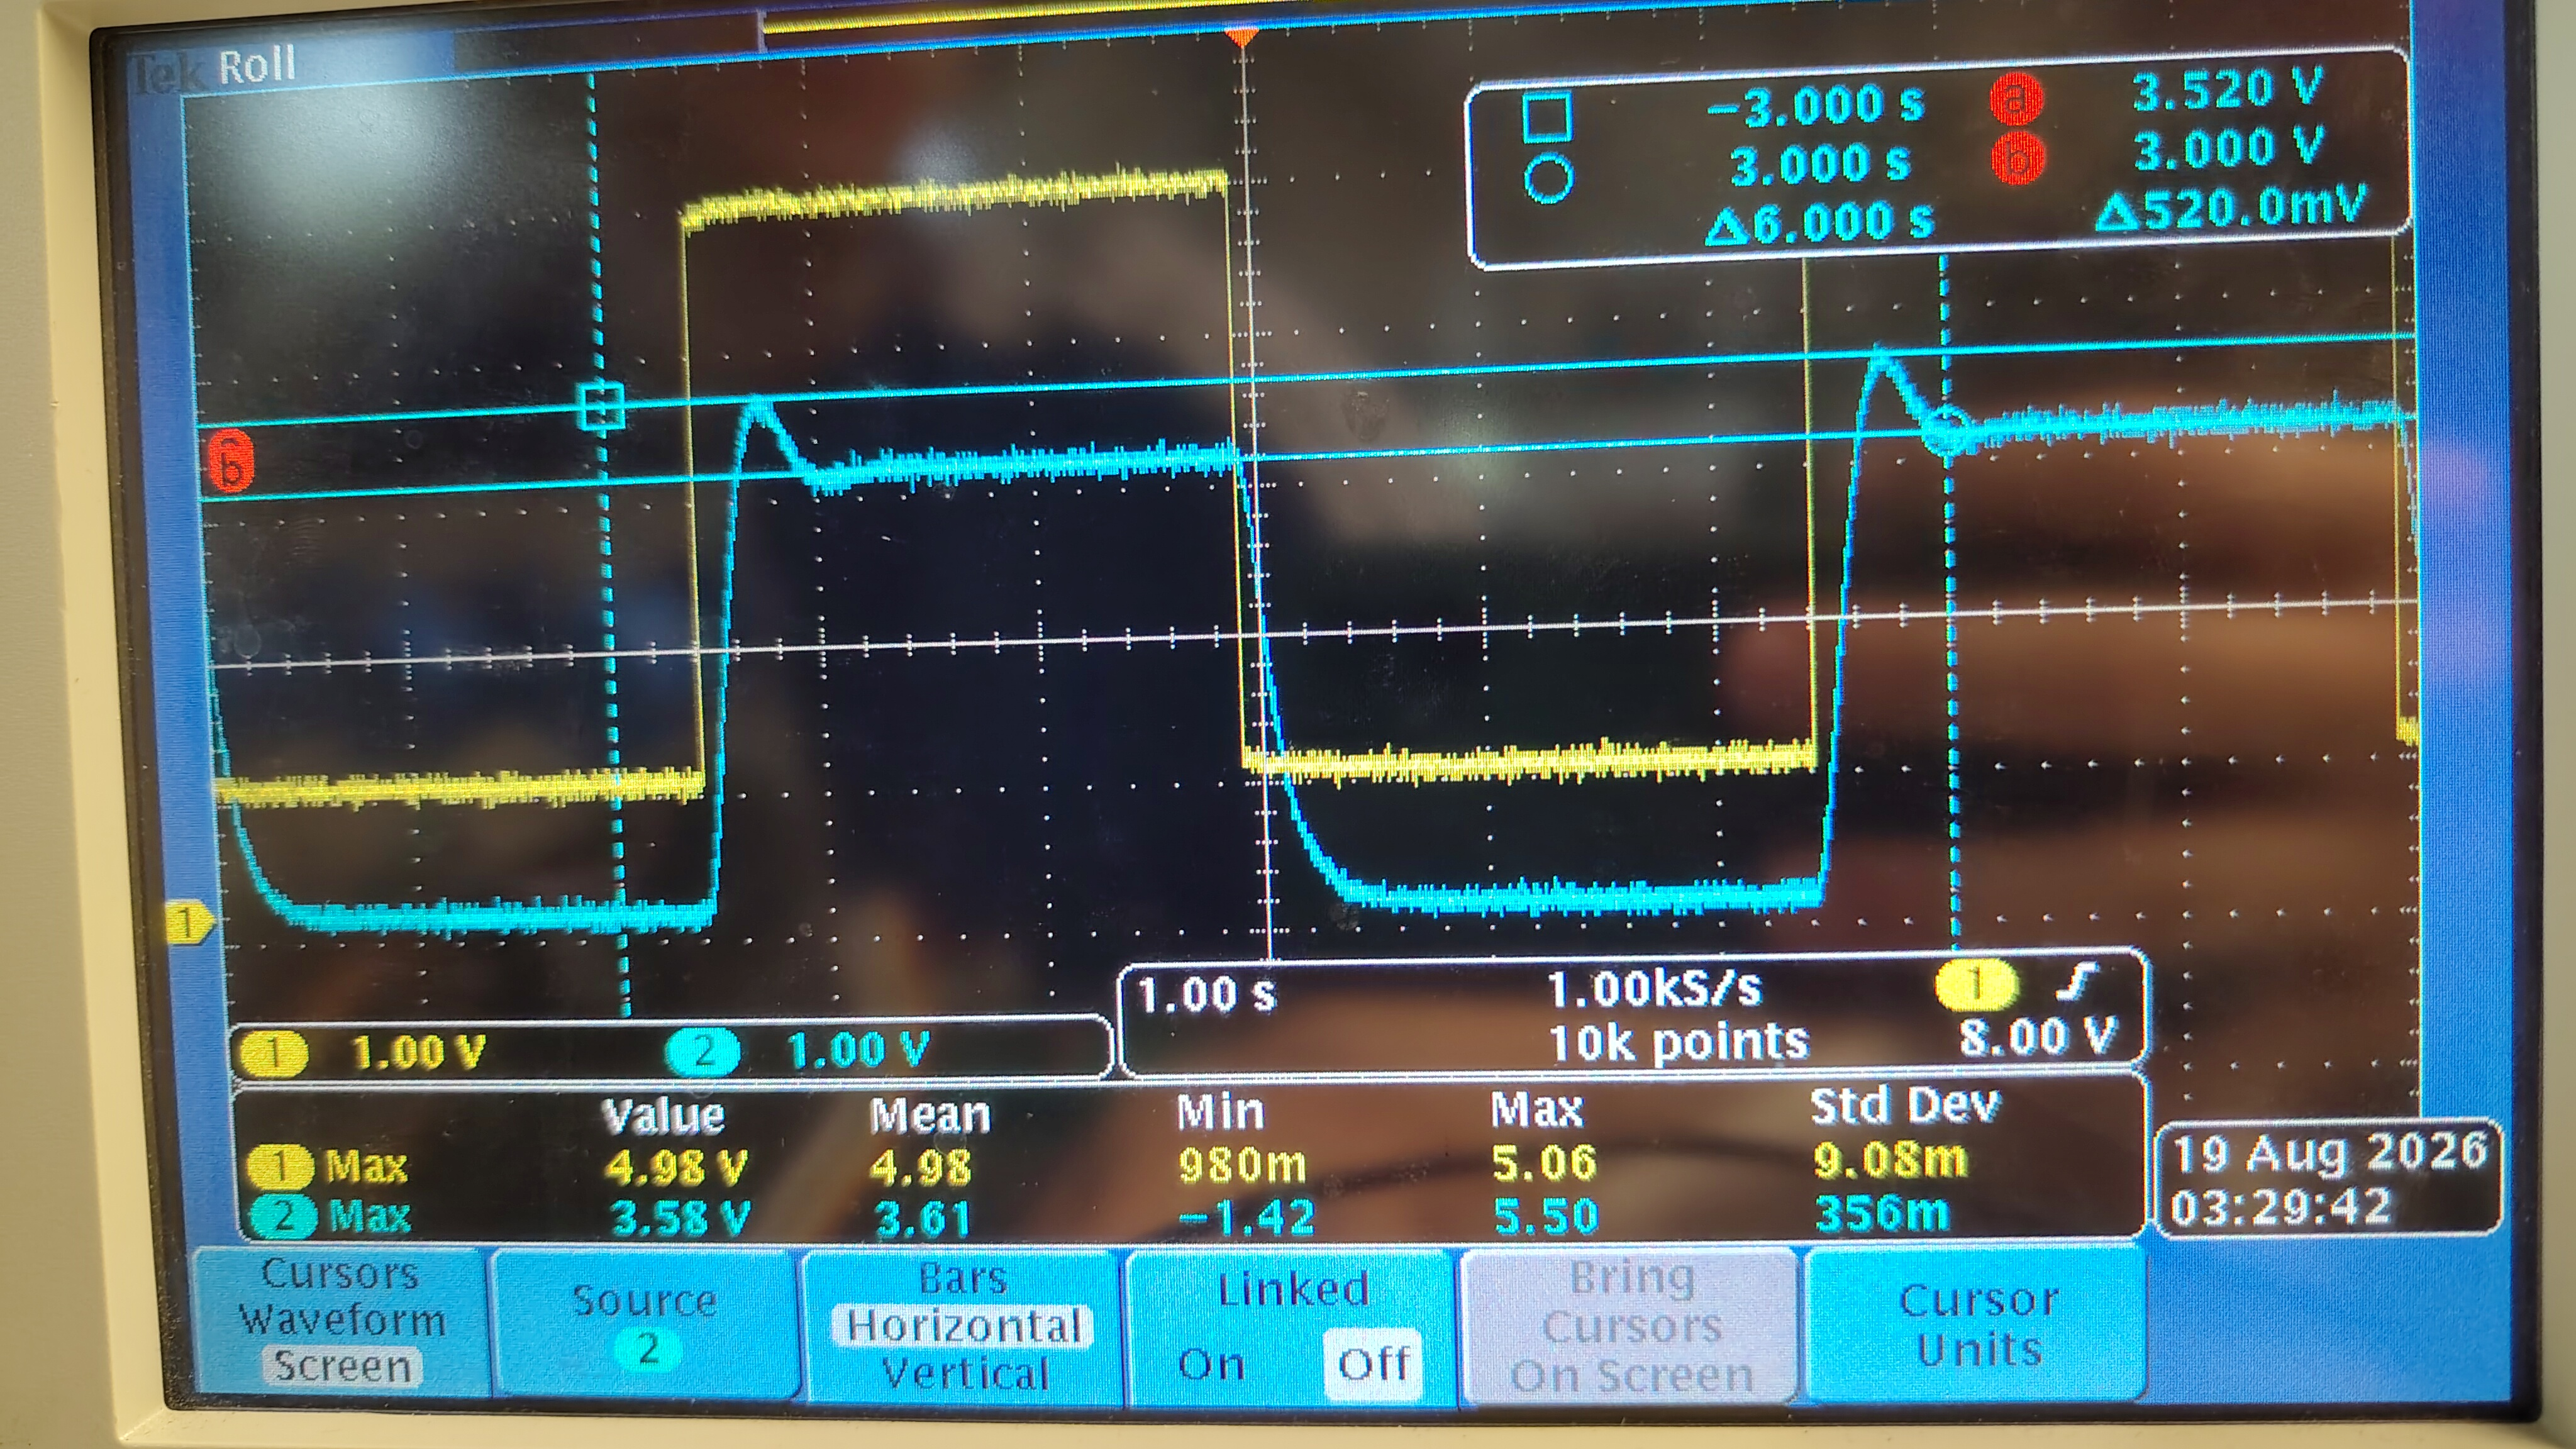
\includegraphics[width=\textwidth]{p_0_skt.jpg}
    \caption{$K_p=0$ Skt}
    \label{fig:p=0}
    \end{subfigure}
    \hfill
    \begin{subfigure}[b]{0.48\textwidth}
    \centering
    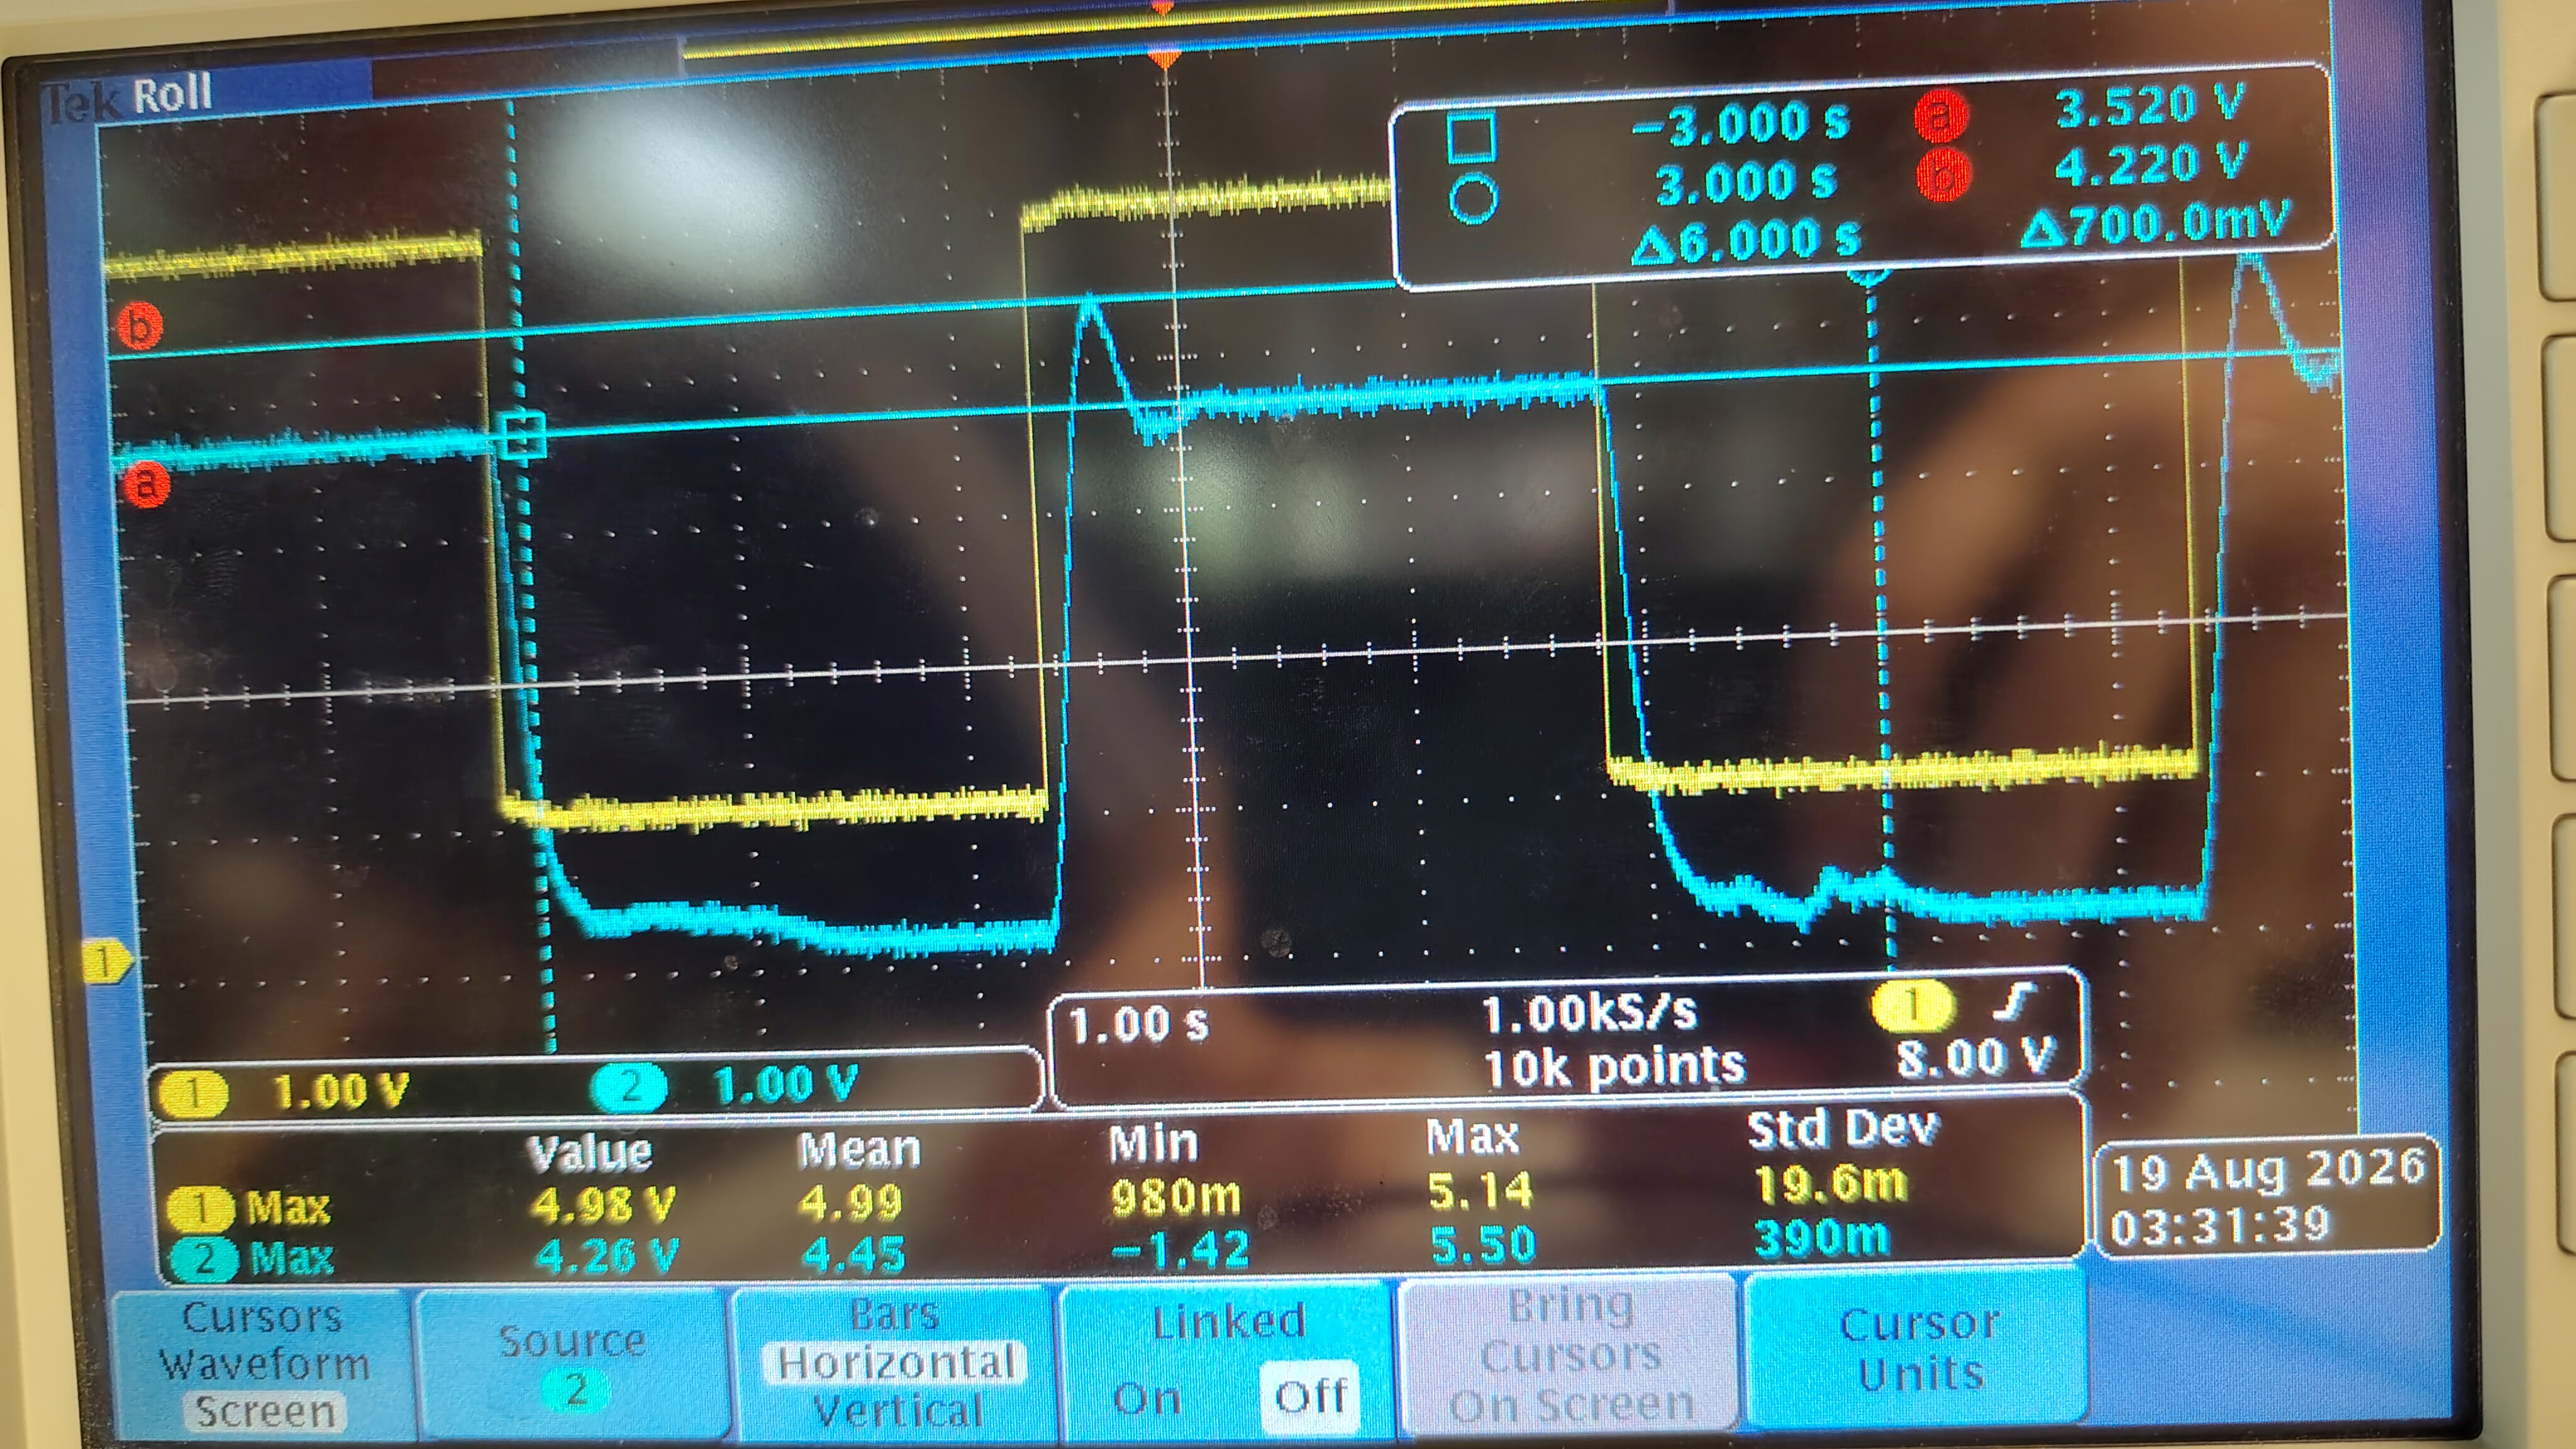
\includegraphics[width=\textwidth]{p_10_skt.jpg}
    \caption{$K_p=10$ Skt}
    \label{fig:p=10}
    \end{subfigure}

    \vspace{0.5cm}

    \begin{subfigure}[b]{0.48\textwidth}
    \centering
    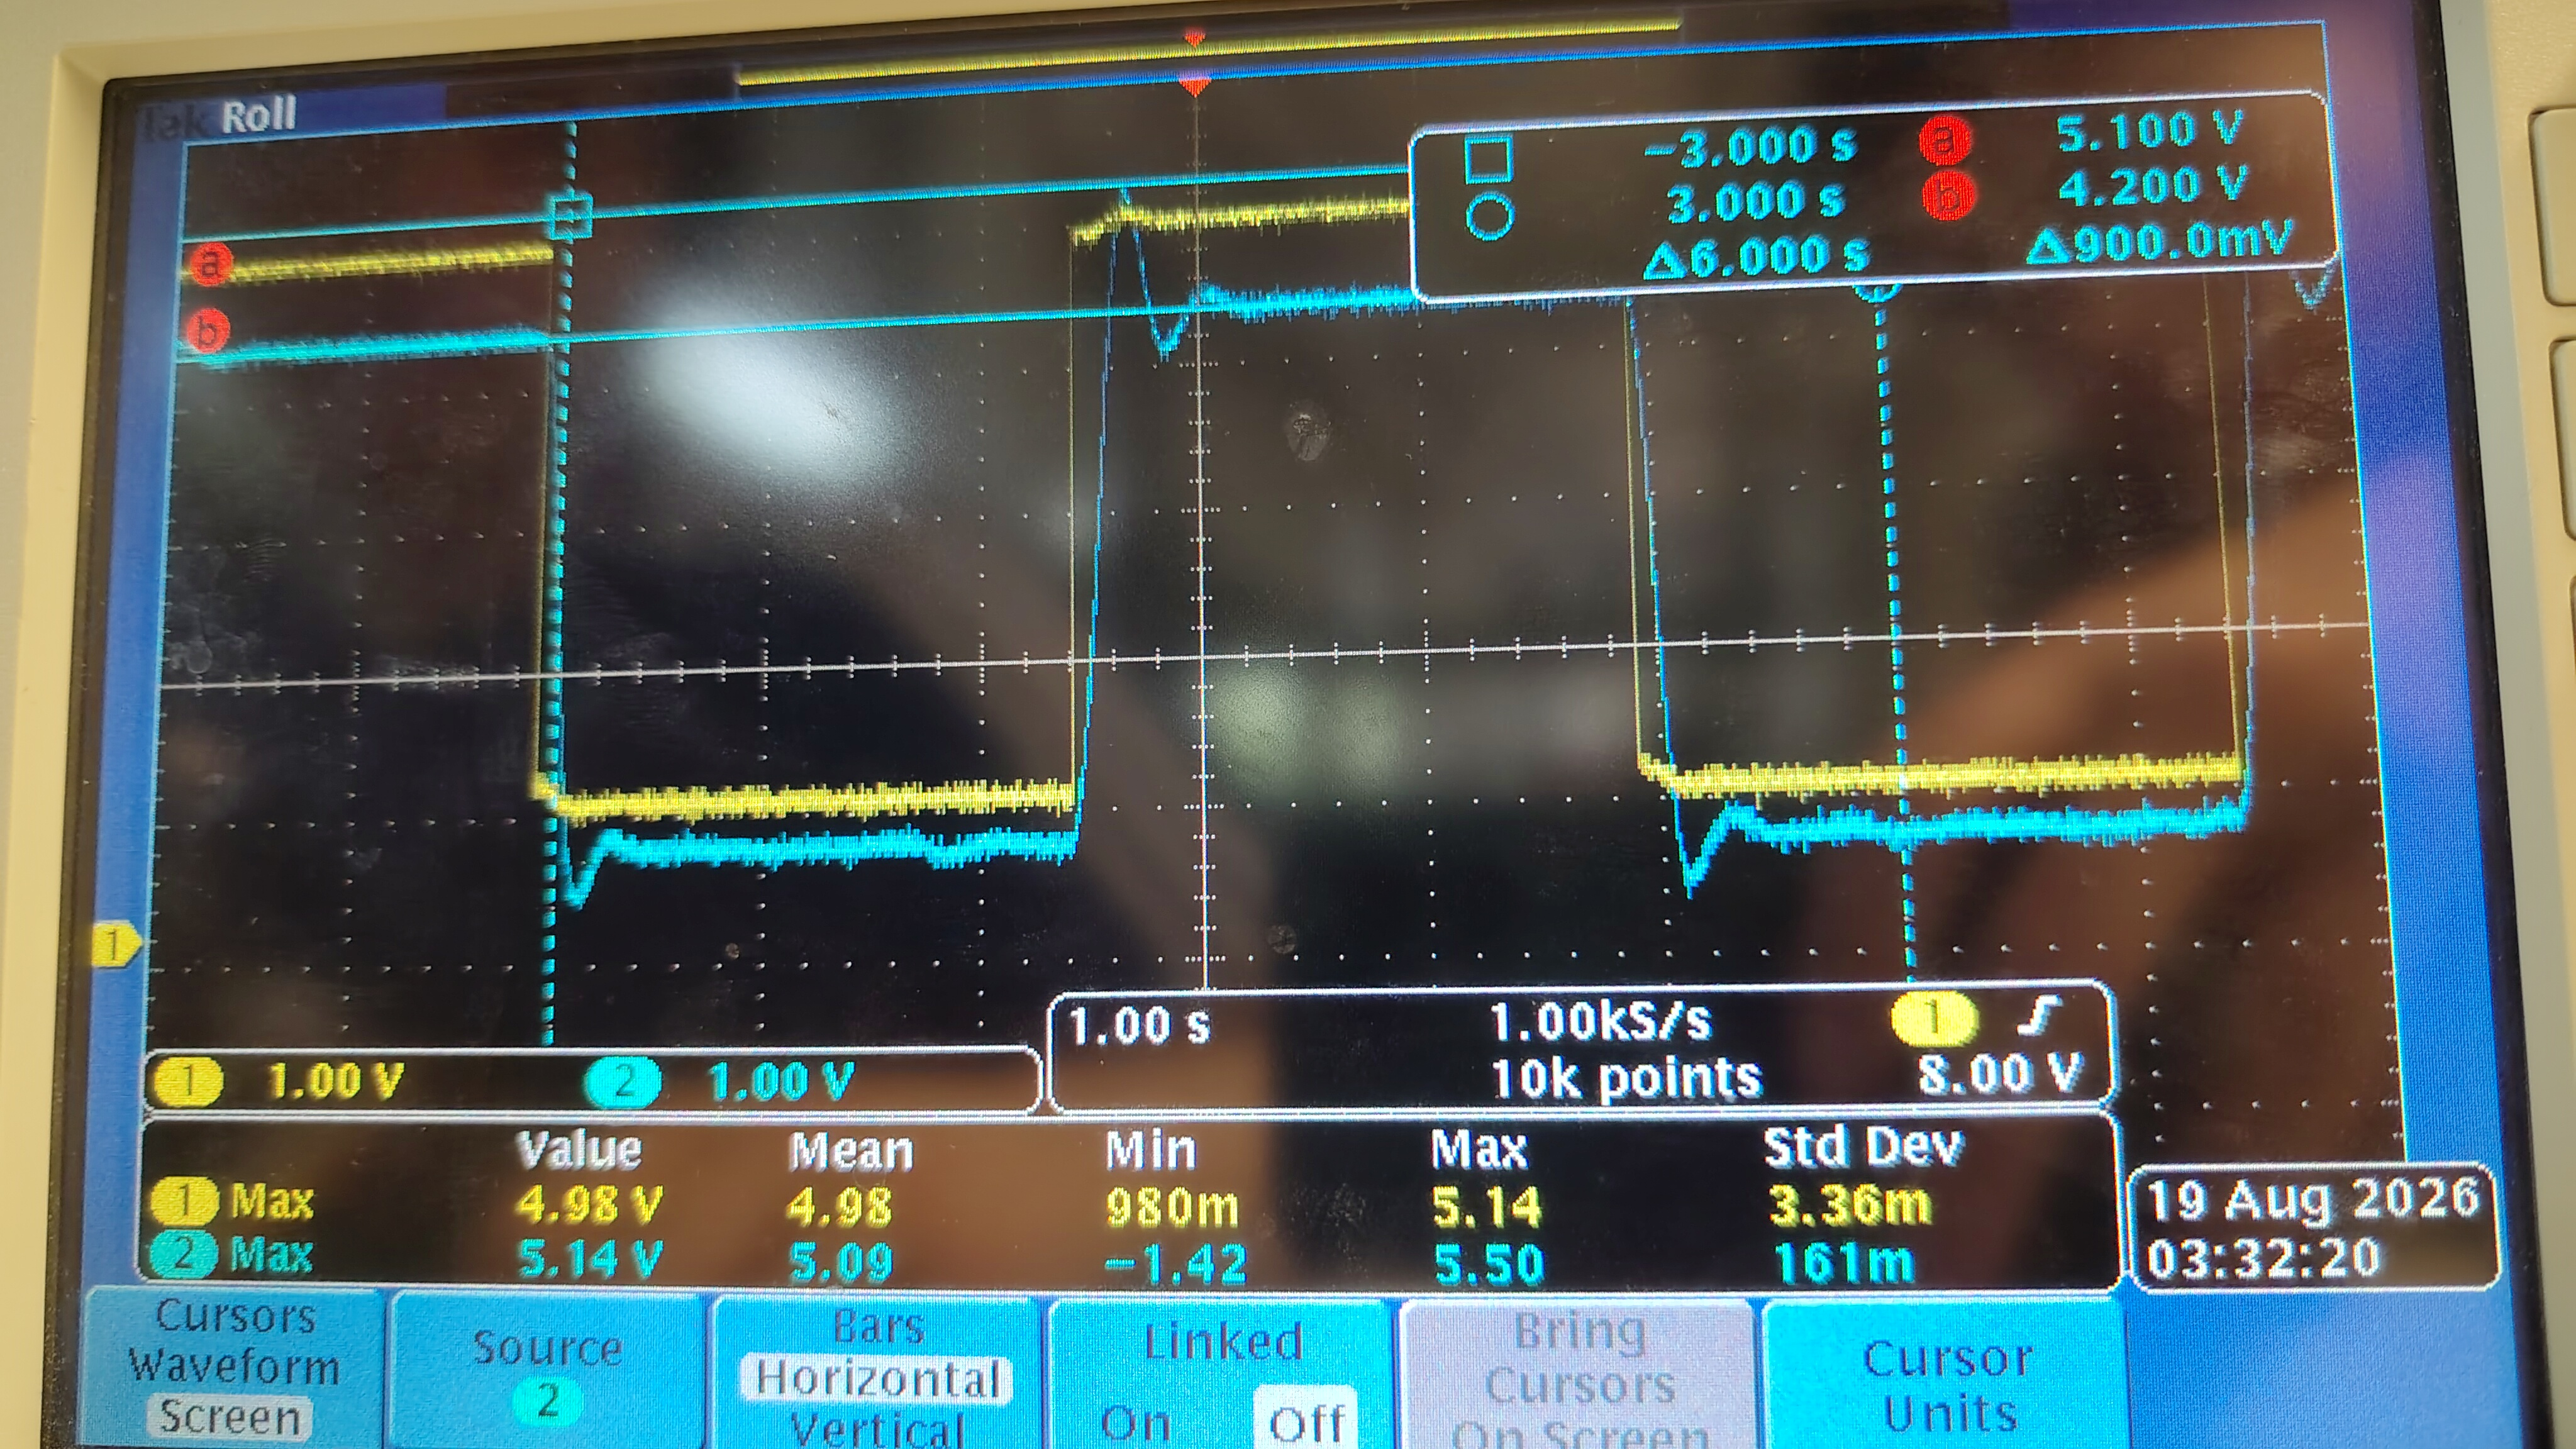
\includegraphics[width=\textwidth]{p_50_skt.jpg}
    \caption{$K_p=50$ Skt}
    \label{fig:p=50}
    \end{subfigure}
    \hfill
    \begin{subfigure}[b]{0.48\textwidth}
    \centering
    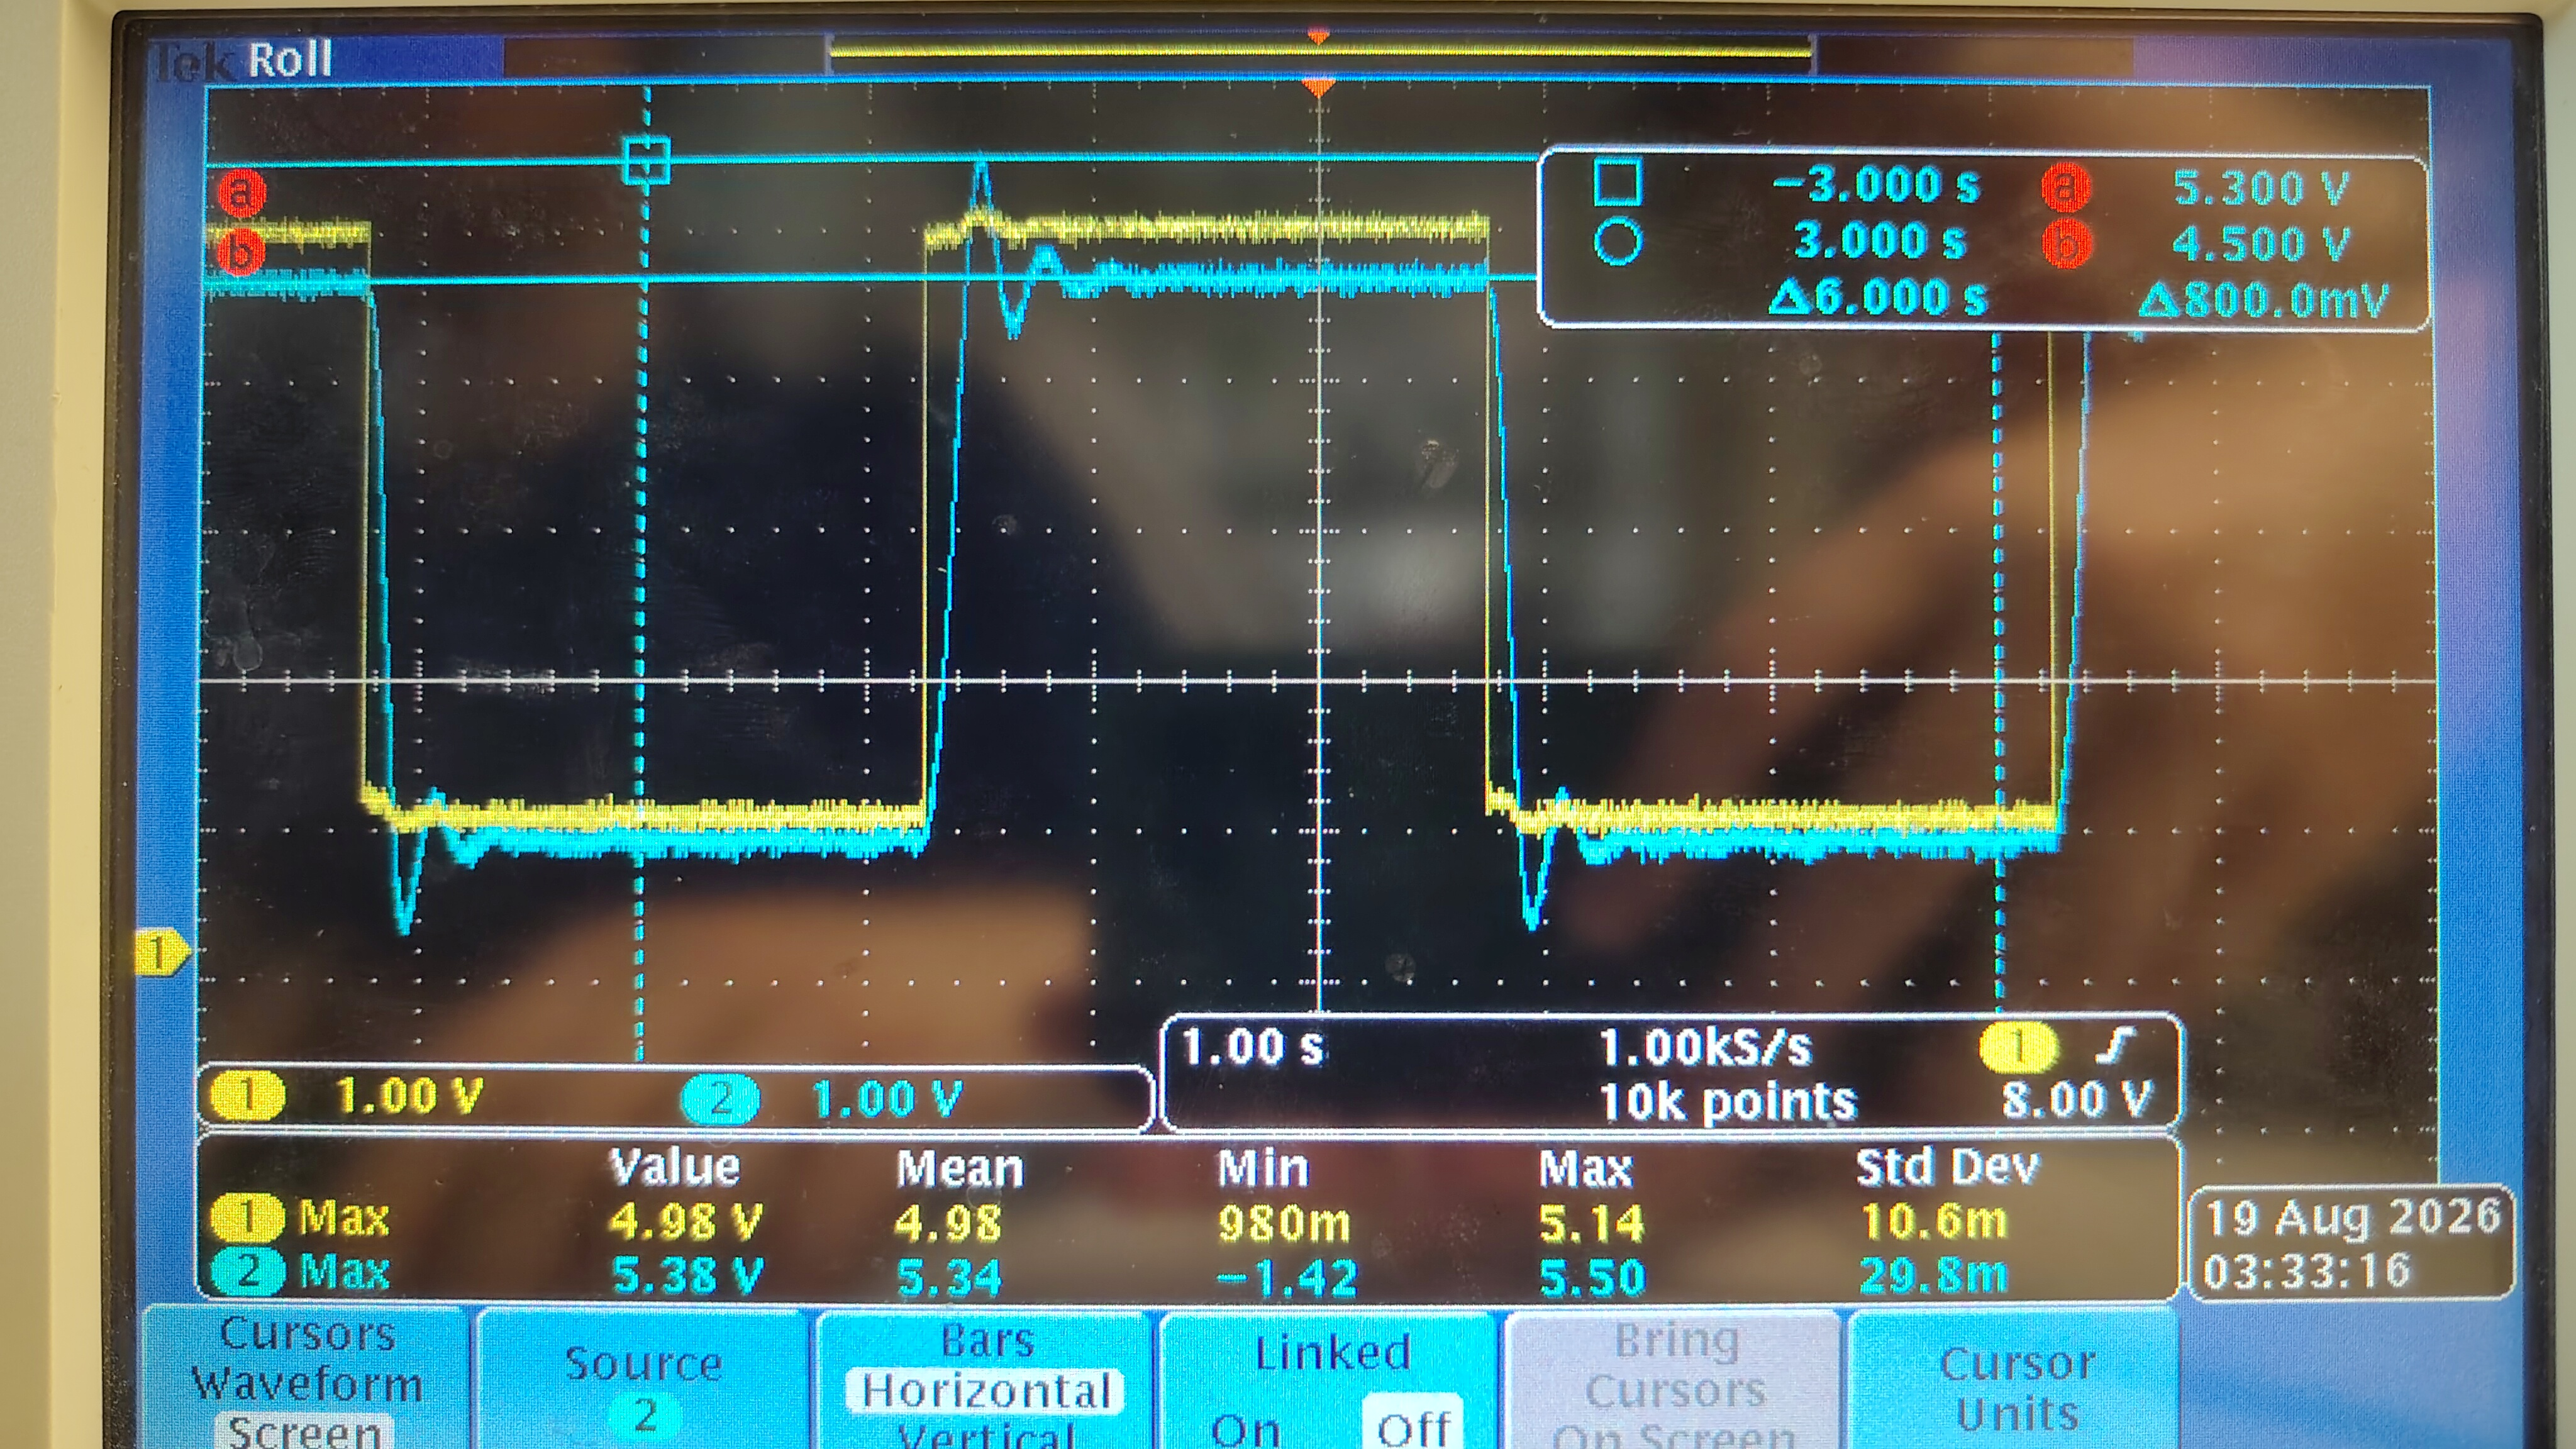
\includegraphics[width=\textwidth]{p_100_skt.jpg}
    \caption{$K_p=100$ Skt}
    \label{fig:p=100}
    \end{subfigure}

    \vspace{0.5cm}

    \begin{subfigure}[b]{0.48\textwidth}
    \centering
    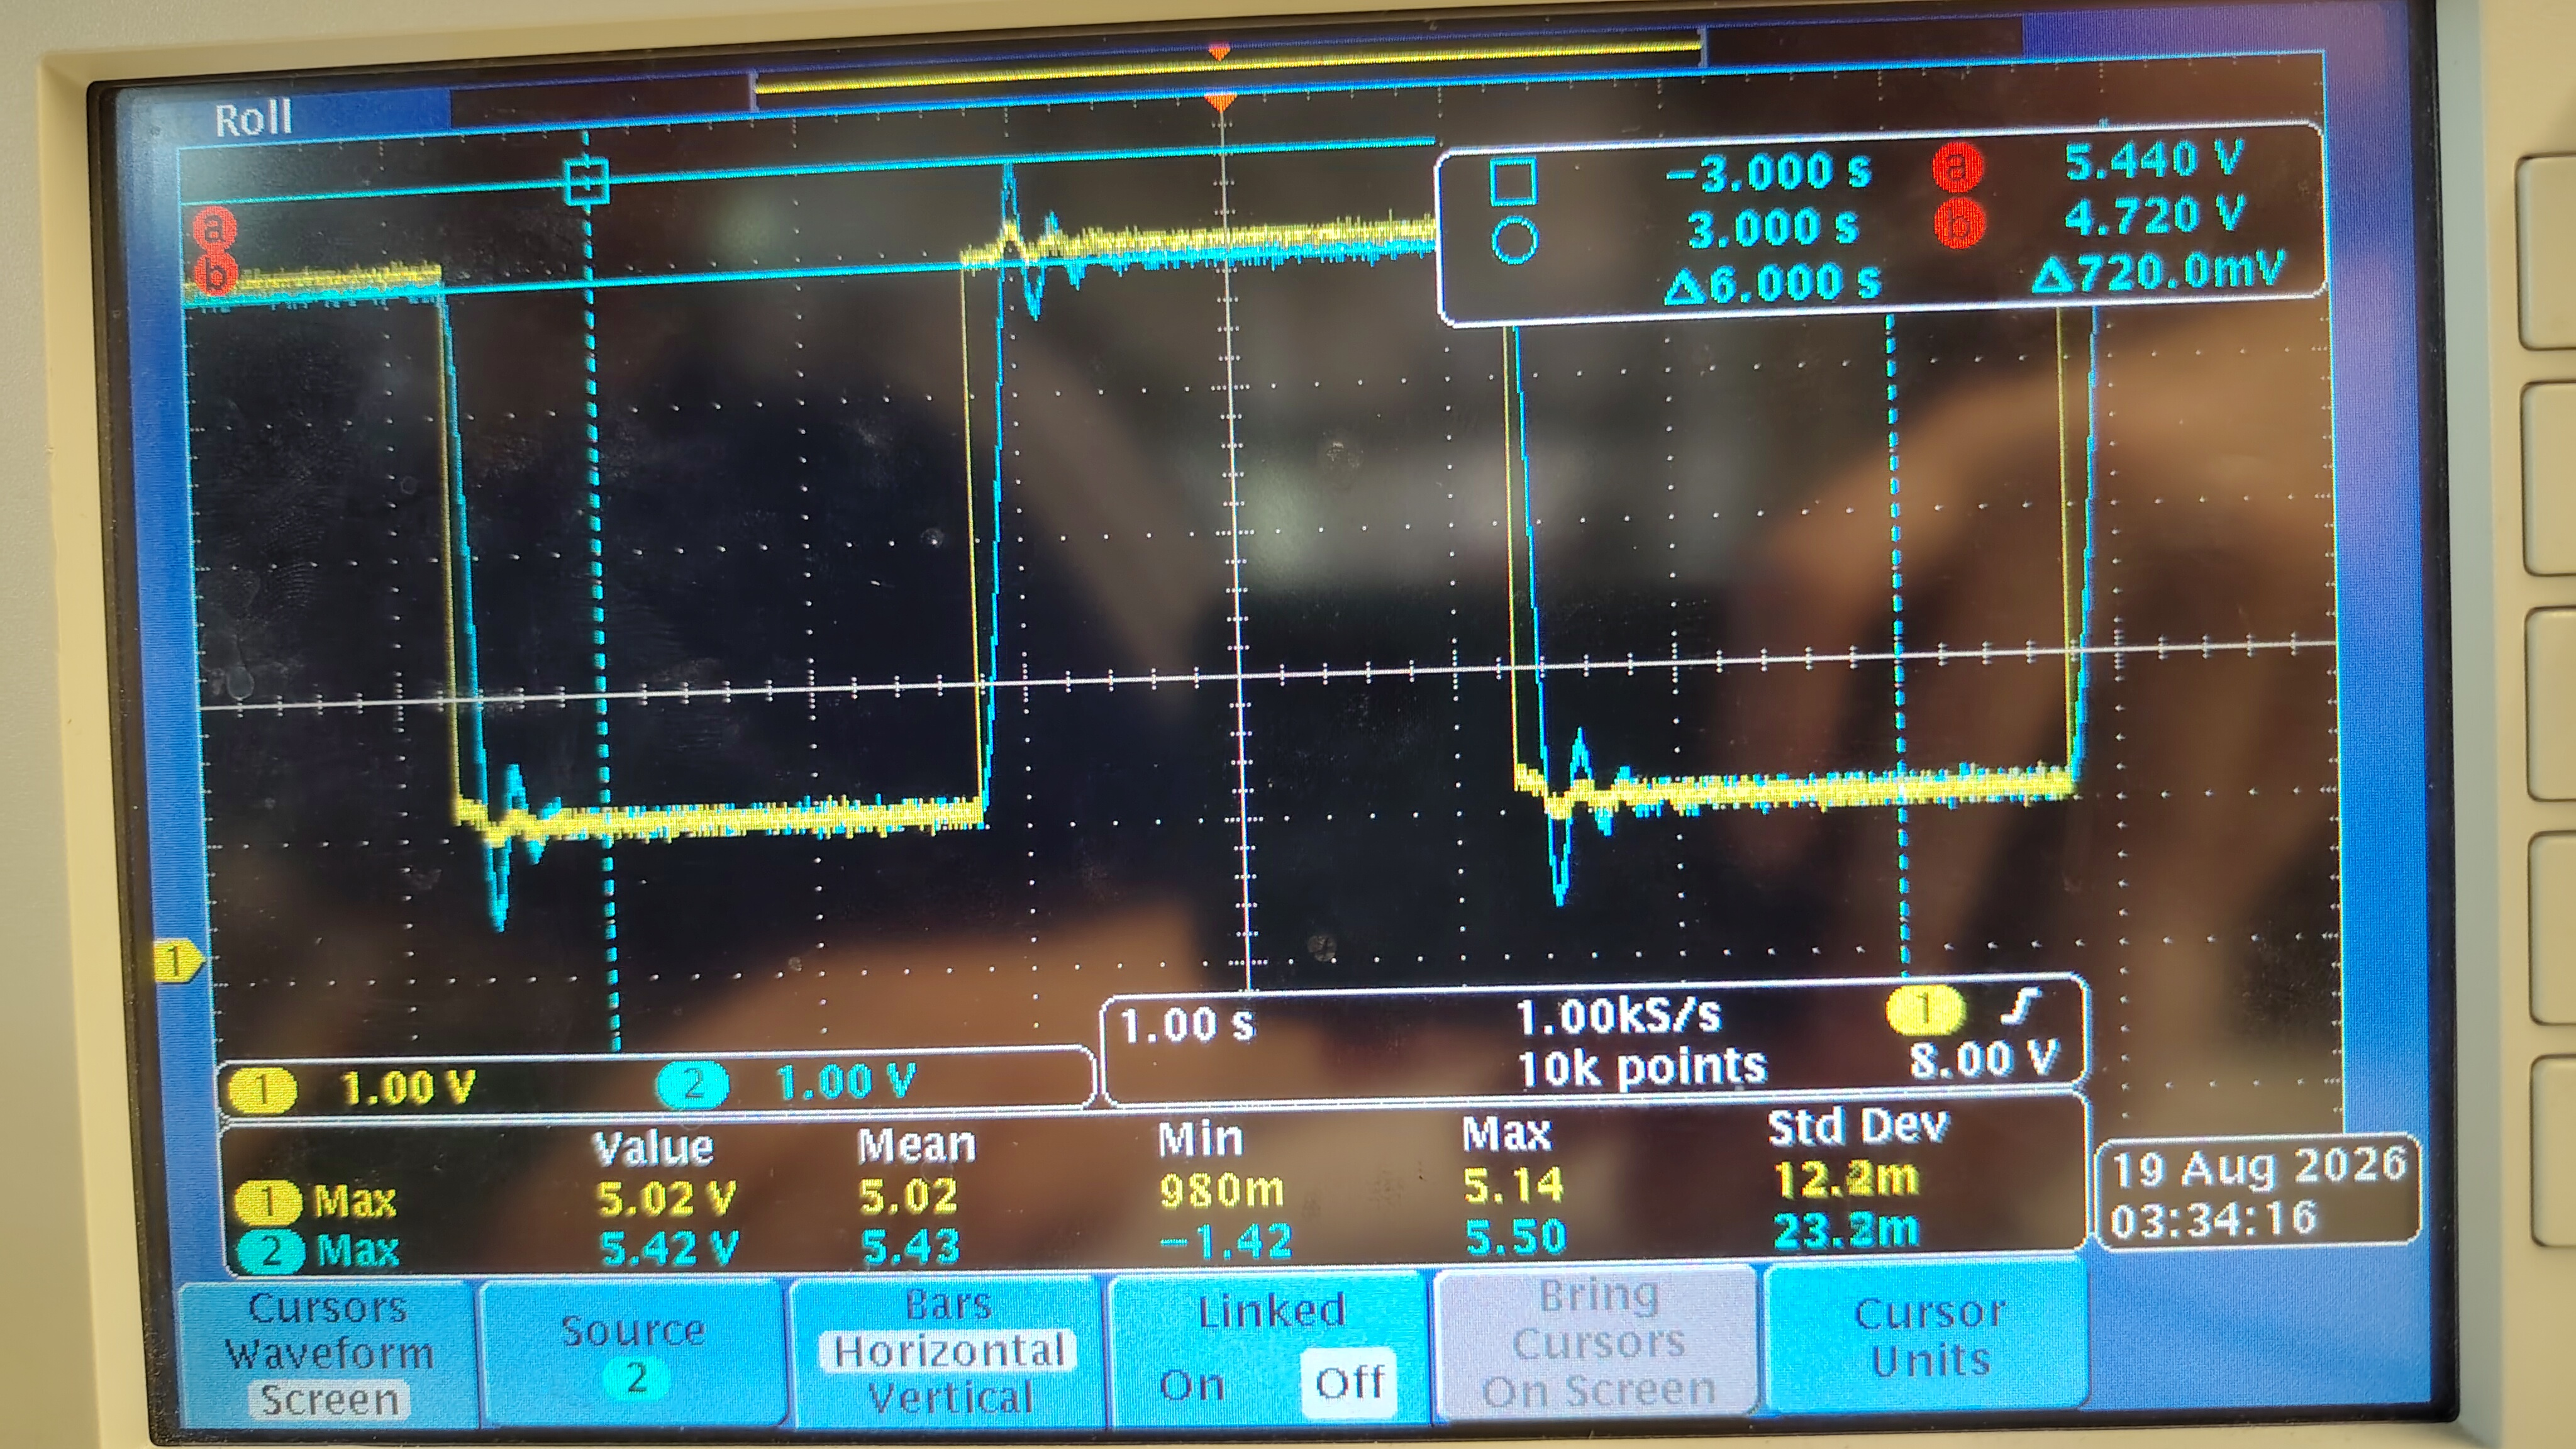
\includegraphics[width=\textwidth]{p_300_skt.jpg}
    \caption{$K_p=300$ Skt}
    \label{fig:p=300}
    \end{subfigure}
    \hfill
    \begin{subfigure}[b]{0.48\textwidth}
    \centering
    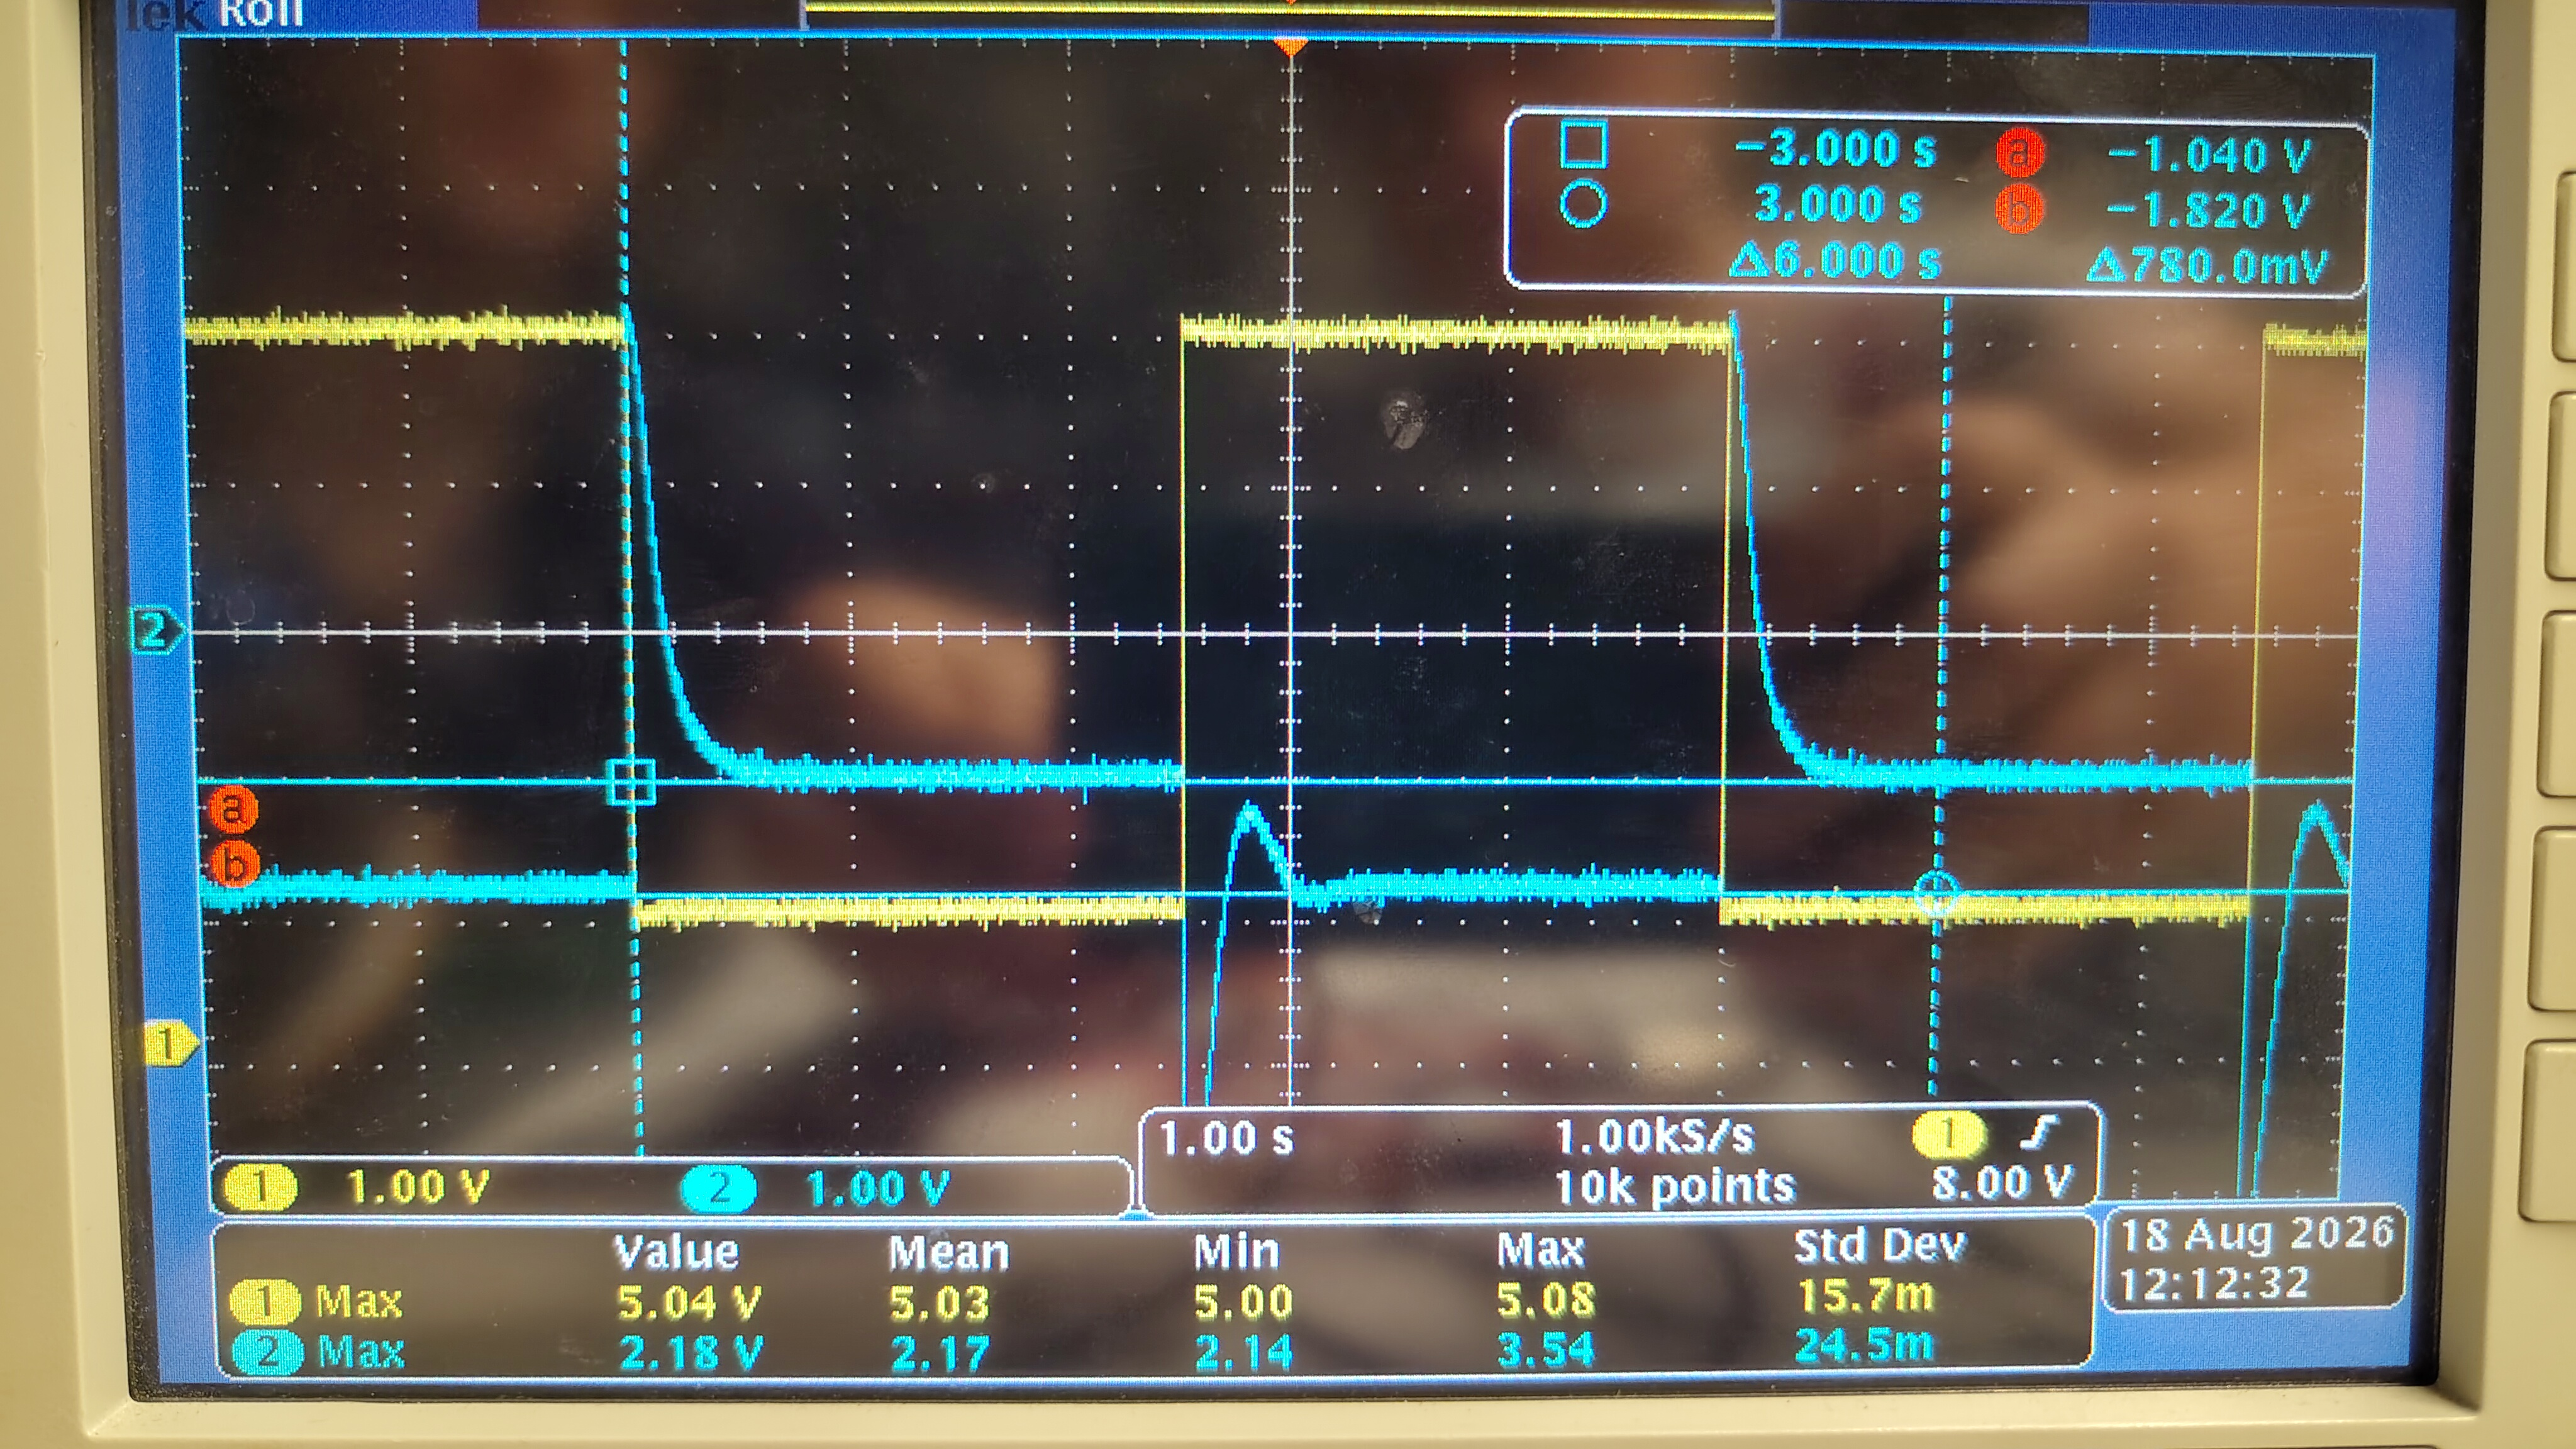
\includegraphics[width=\textwidth]{p_klein_5_skt.jpg}
    \caption{$K_p=5$ Skt, in Blau: Ist-Soll}
    \label{fig:p=5_ist-soll}
    \end{subfigure}
    \caption{P-Regler mit unterschiedlichen $K_p$, in (f) ist zusätzlich ist-soll abgebildet für $K_p=5$ Skt}
    \label{fig:K_p-Regler}
\end{figure}

Man erkennt in \Cref{fig:K_p-Regler} die Anpassung des Motors an das Rechtecksignal (in Blau, Rechtecksignal in Gelb) für unterschiedliche Proportionalbeiwerte $K_p$. In \Cref{fig:p=0} sieht man die Einstellung mit minimalem $K_p$. Dabei ist die Motordrehzahl stets kleiner als das Soll. Bei kleinen \(K_p\) erkennt man, dass das Soll bei der kleineren Amplitude auf Null sinkt und somit der Motor stehen bleibt. Beim Sprung im Rechtecksignal auf die höhere Amplitude wird auch der 
Motor hochgeregelt. Dabei gibt es zunächst einen Peak, der immer höher ist, als das anschließend erreichte Niveau der P-Regelung. Diese Überschwingungen werden größer, mit zunehmendem \(K_p\). Außerdem werden bei steigendem \(K_p\) auch mehr Amplituden der Überschwingung sichtbar. Folglich wird ein stabiler Wert erst später erreicht. Die stationäre Genauigkeit betreffend erkennt man in den Aufnahmen gut, dass diese bei steigendem $K_p$ verbessert wird. Genau erreicht wird das Niveau jedoch nicht, wie man auch bei hohen $K_p$ erkennen kann, aber es nähert sich schon gut an.
Keinen Unterschied sieht man bei der Regelgeschwindigkeit, also der Zeitdauer nach einer Sollwert-Änderung bis zu einer Regel-Anpassung durch den P-Regler.
In \Cref{fig:p=5_ist-soll} erkennt man zusätzlich noch den Ist-Soll-Verlauf. Hierbei wurde die Null auf die Mitte der Anzeige verschoben. Man sieht, dass die Abweichung direkt nach der Sollwert-Anpassung maximal wird, weil der P-Regler natürlich nicht instantan regelt. Ansonsten lässt sich dem Oszilloskop-Bild entnehmen, dass der Soll-Wert sonst immer größer als der Ist-Wert ist.

\paragraph{PI-Regelung} Hier ist nun der P- und der I-Anteil aktiviert, der D-Anteil bleibt weiterhin ausgeschaltet.

\begin{figure}[htbp]
    \begin{subfigure}[b]{0.48\textwidth}
    \centering
    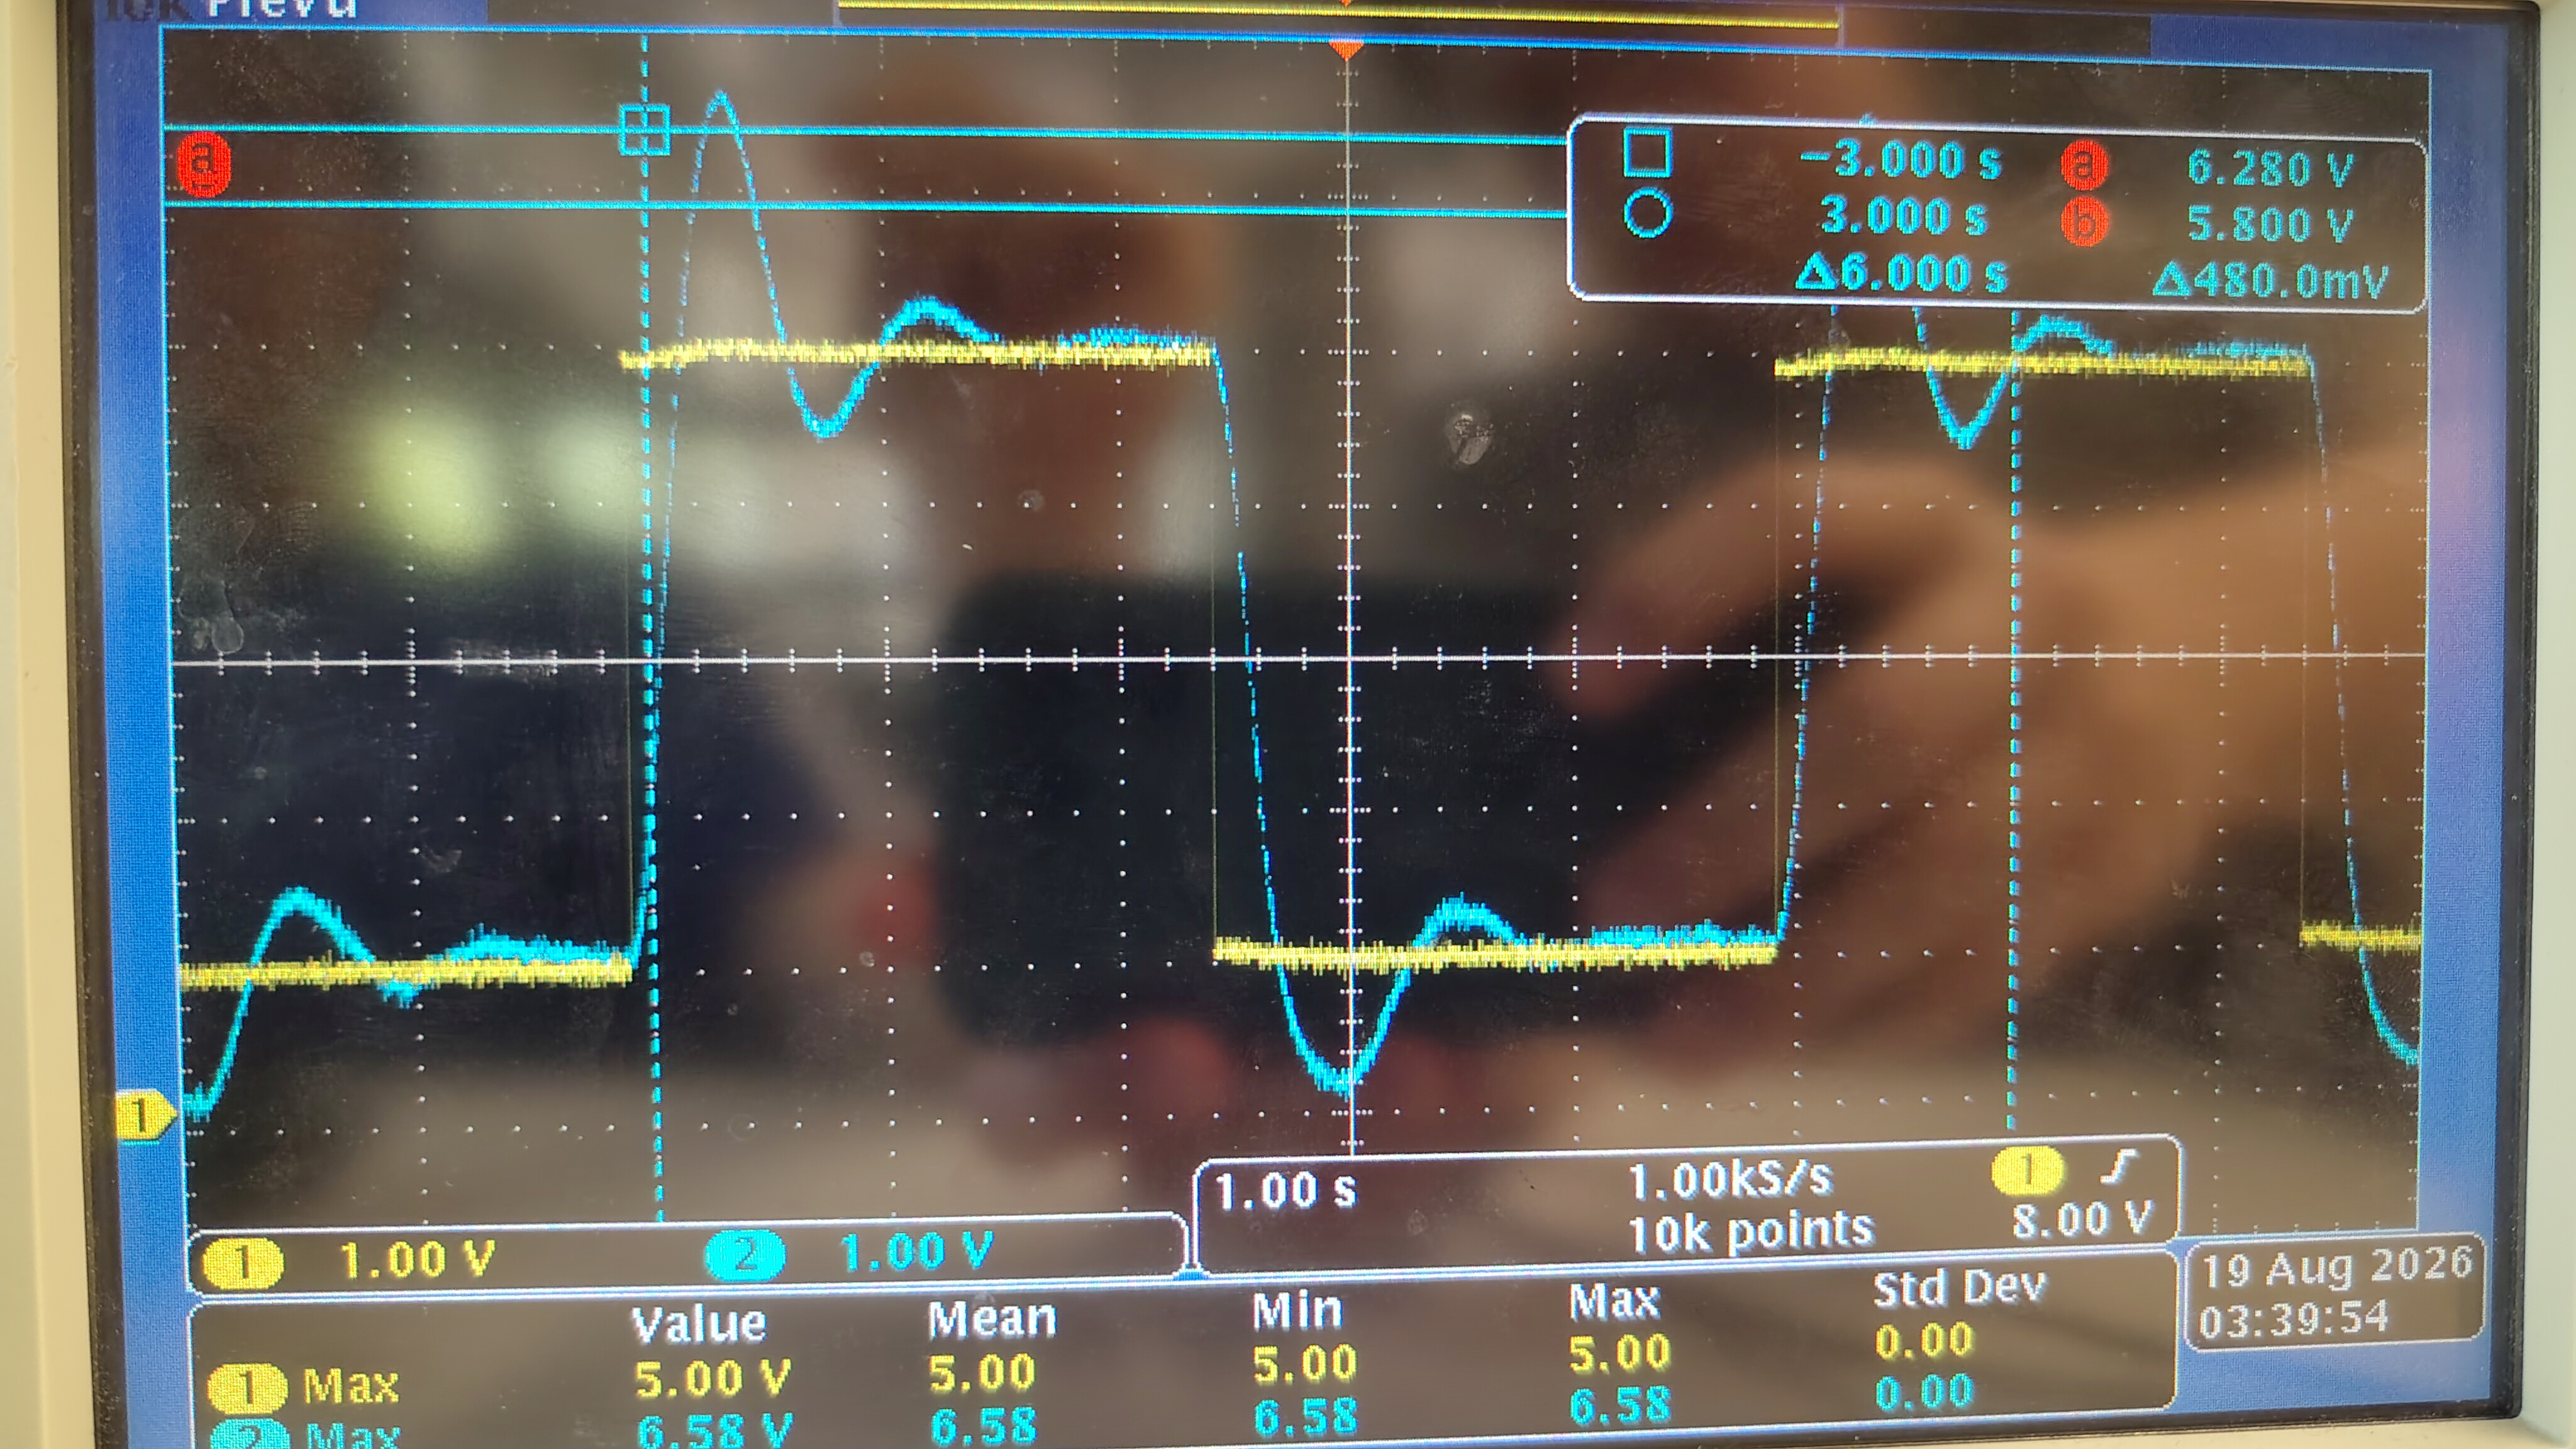
\includegraphics[width=\textwidth]{P_I_0.jpg}
    \caption{$K_p=0$ Skt, $K_I=0$ Skt}
    \label{fig:p=0_i=0}
    \end{subfigure}
    \hfill
    \begin{subfigure}[b]{0.48\textwidth}
    \centering
    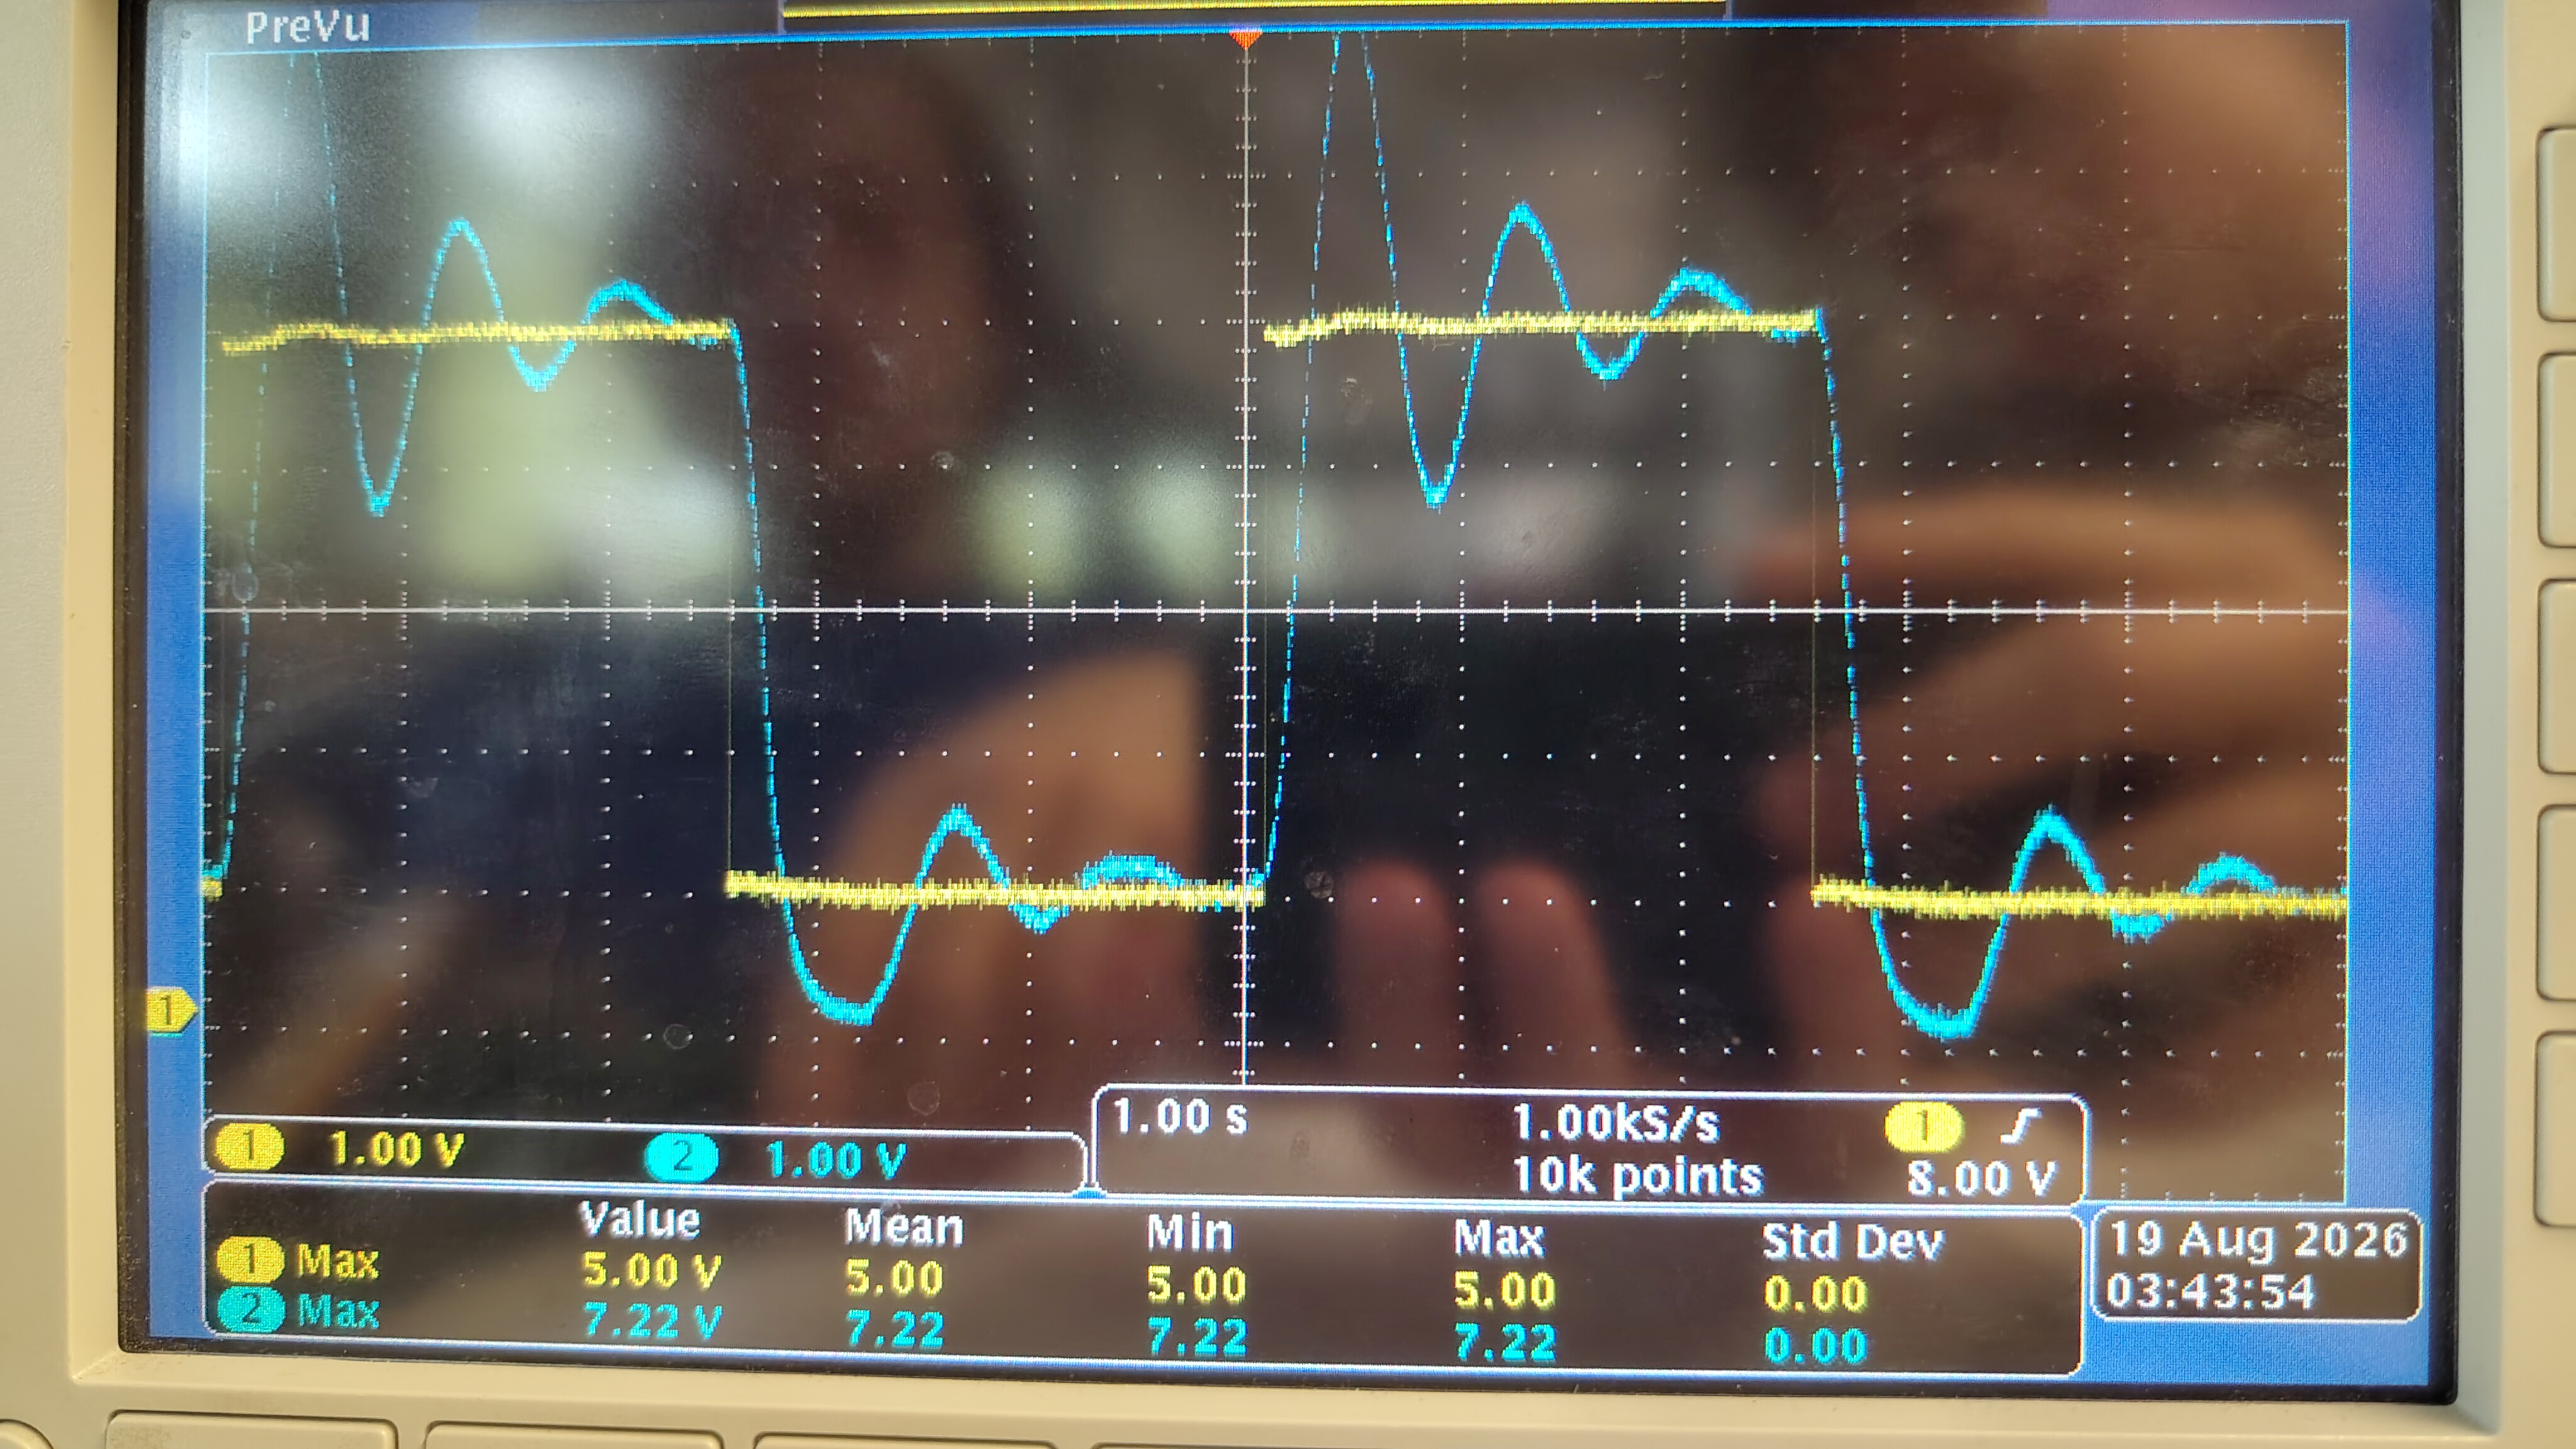
\includegraphics[width=\textwidth]{P_0_I_5.jpg}
    \caption{$K_p=0$ Skt, $K_I=5$ Skt}
    \label{fig:p=0_i=5}
    \end{subfigure}
    \vspace{0.5cm}
    \begin{subfigure}[b]{0.48\textwidth}
    \centering
    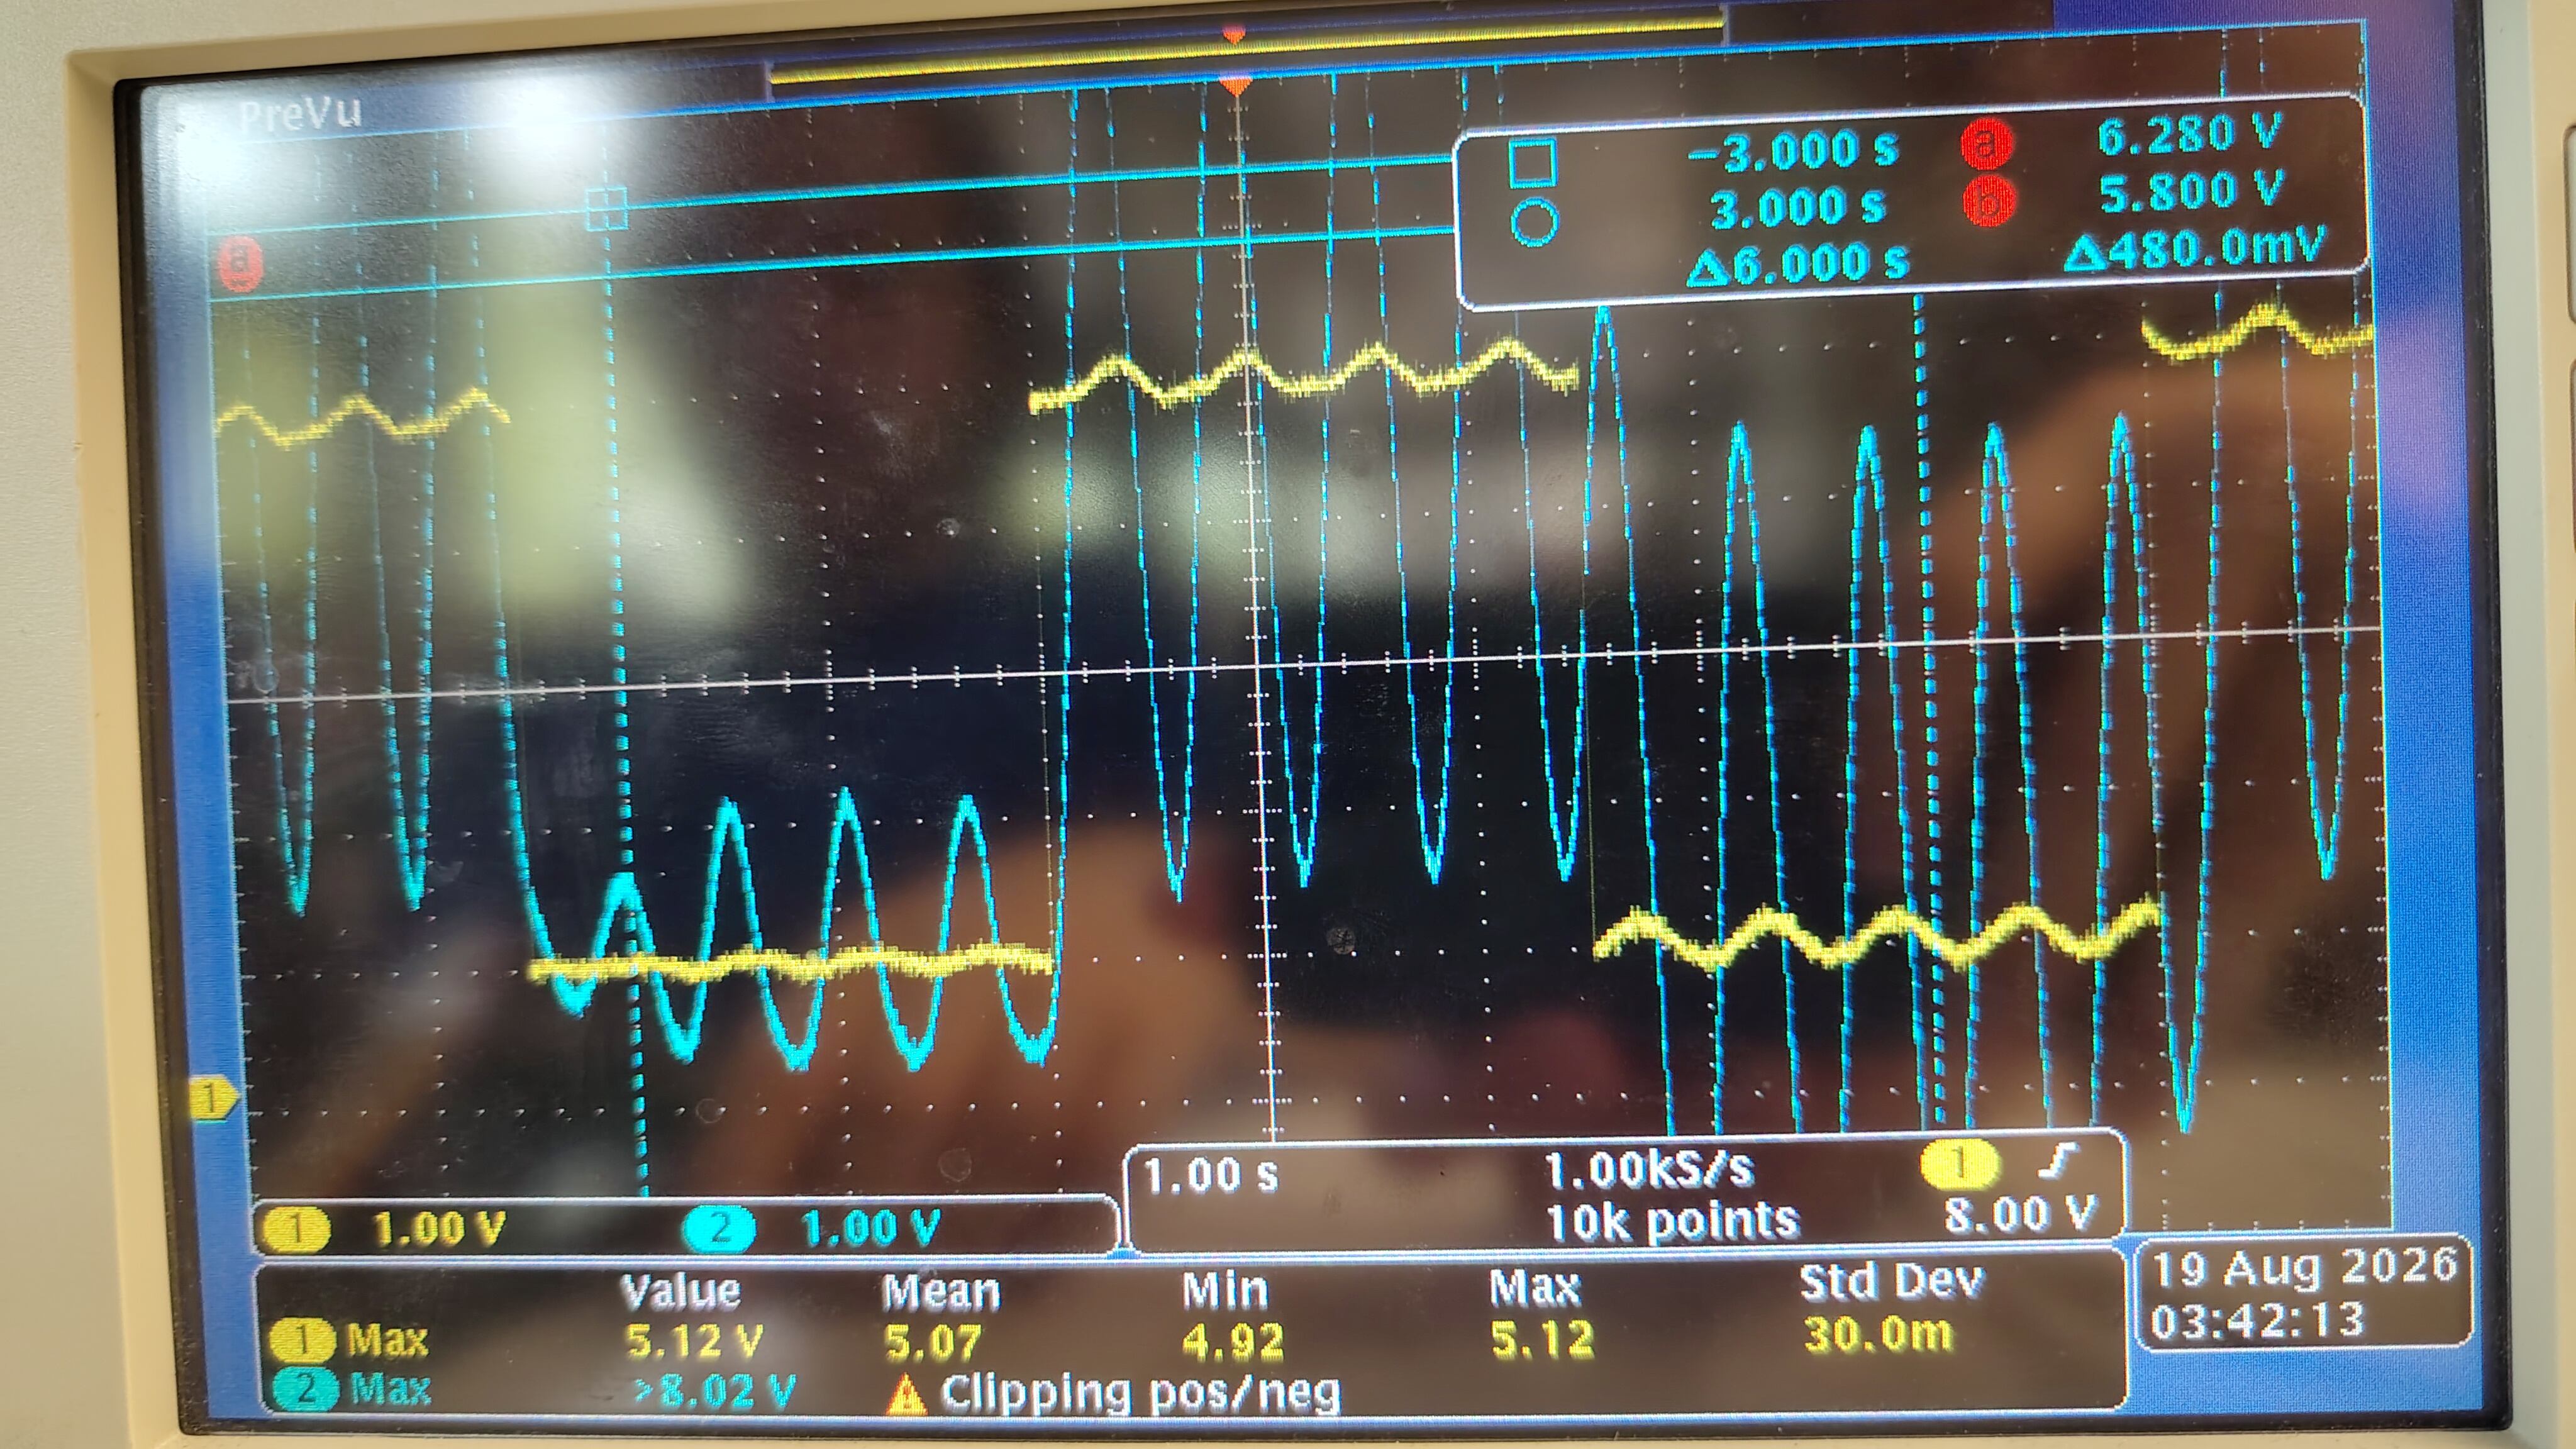
\includegraphics[width=\textwidth]{P_0_I_50.jpg}
    \caption{$K_p=0$ Skt, $K_I=50$ Skt}
    \label{fig:p=0_i=50}
    \end{subfigure}
    \hfill
    \begin{subfigure}[b]{0.48\textwidth}
    \centering
    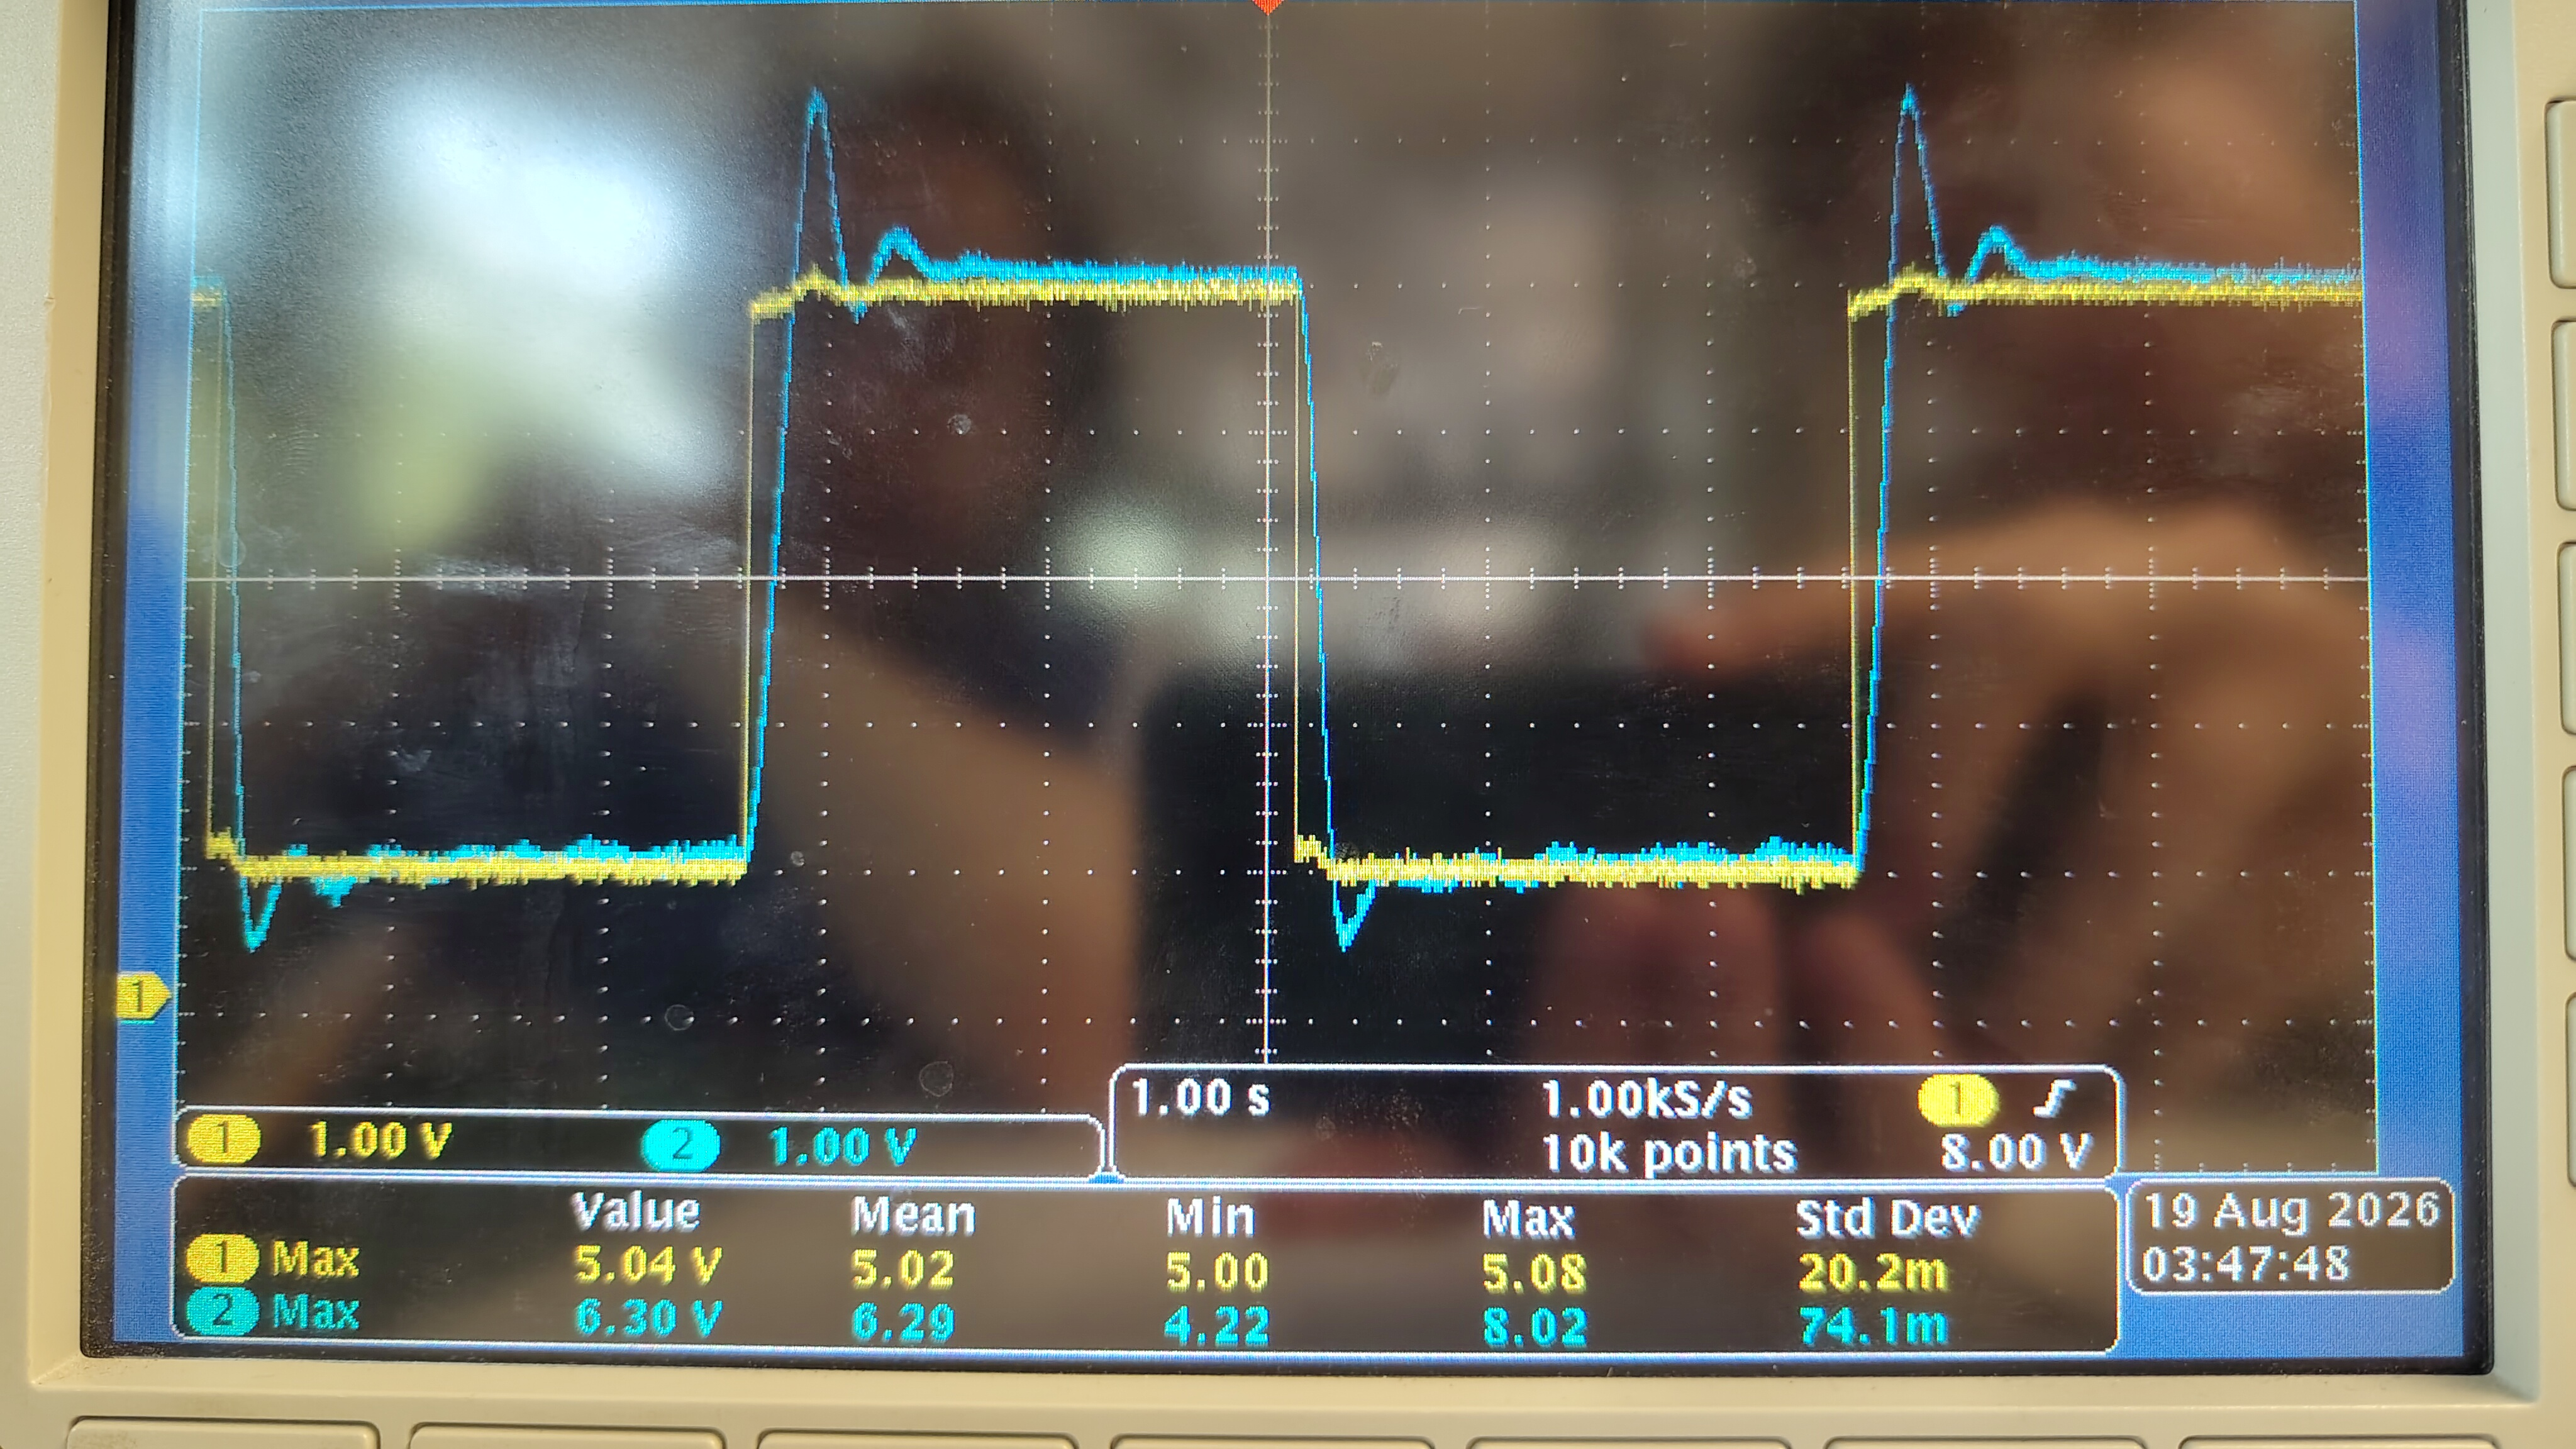
\includegraphics[width=\textwidth]{P_50_I_5.jpg}
    \caption{$K_p=50$ Skt, $K_I=5$ Skt}
    \label{fig:p=50_i=5}
    \end{subfigure}
    \vspace{0.5cm}
    \begin{subfigure}[b]{0.48\textwidth}
    \centering
    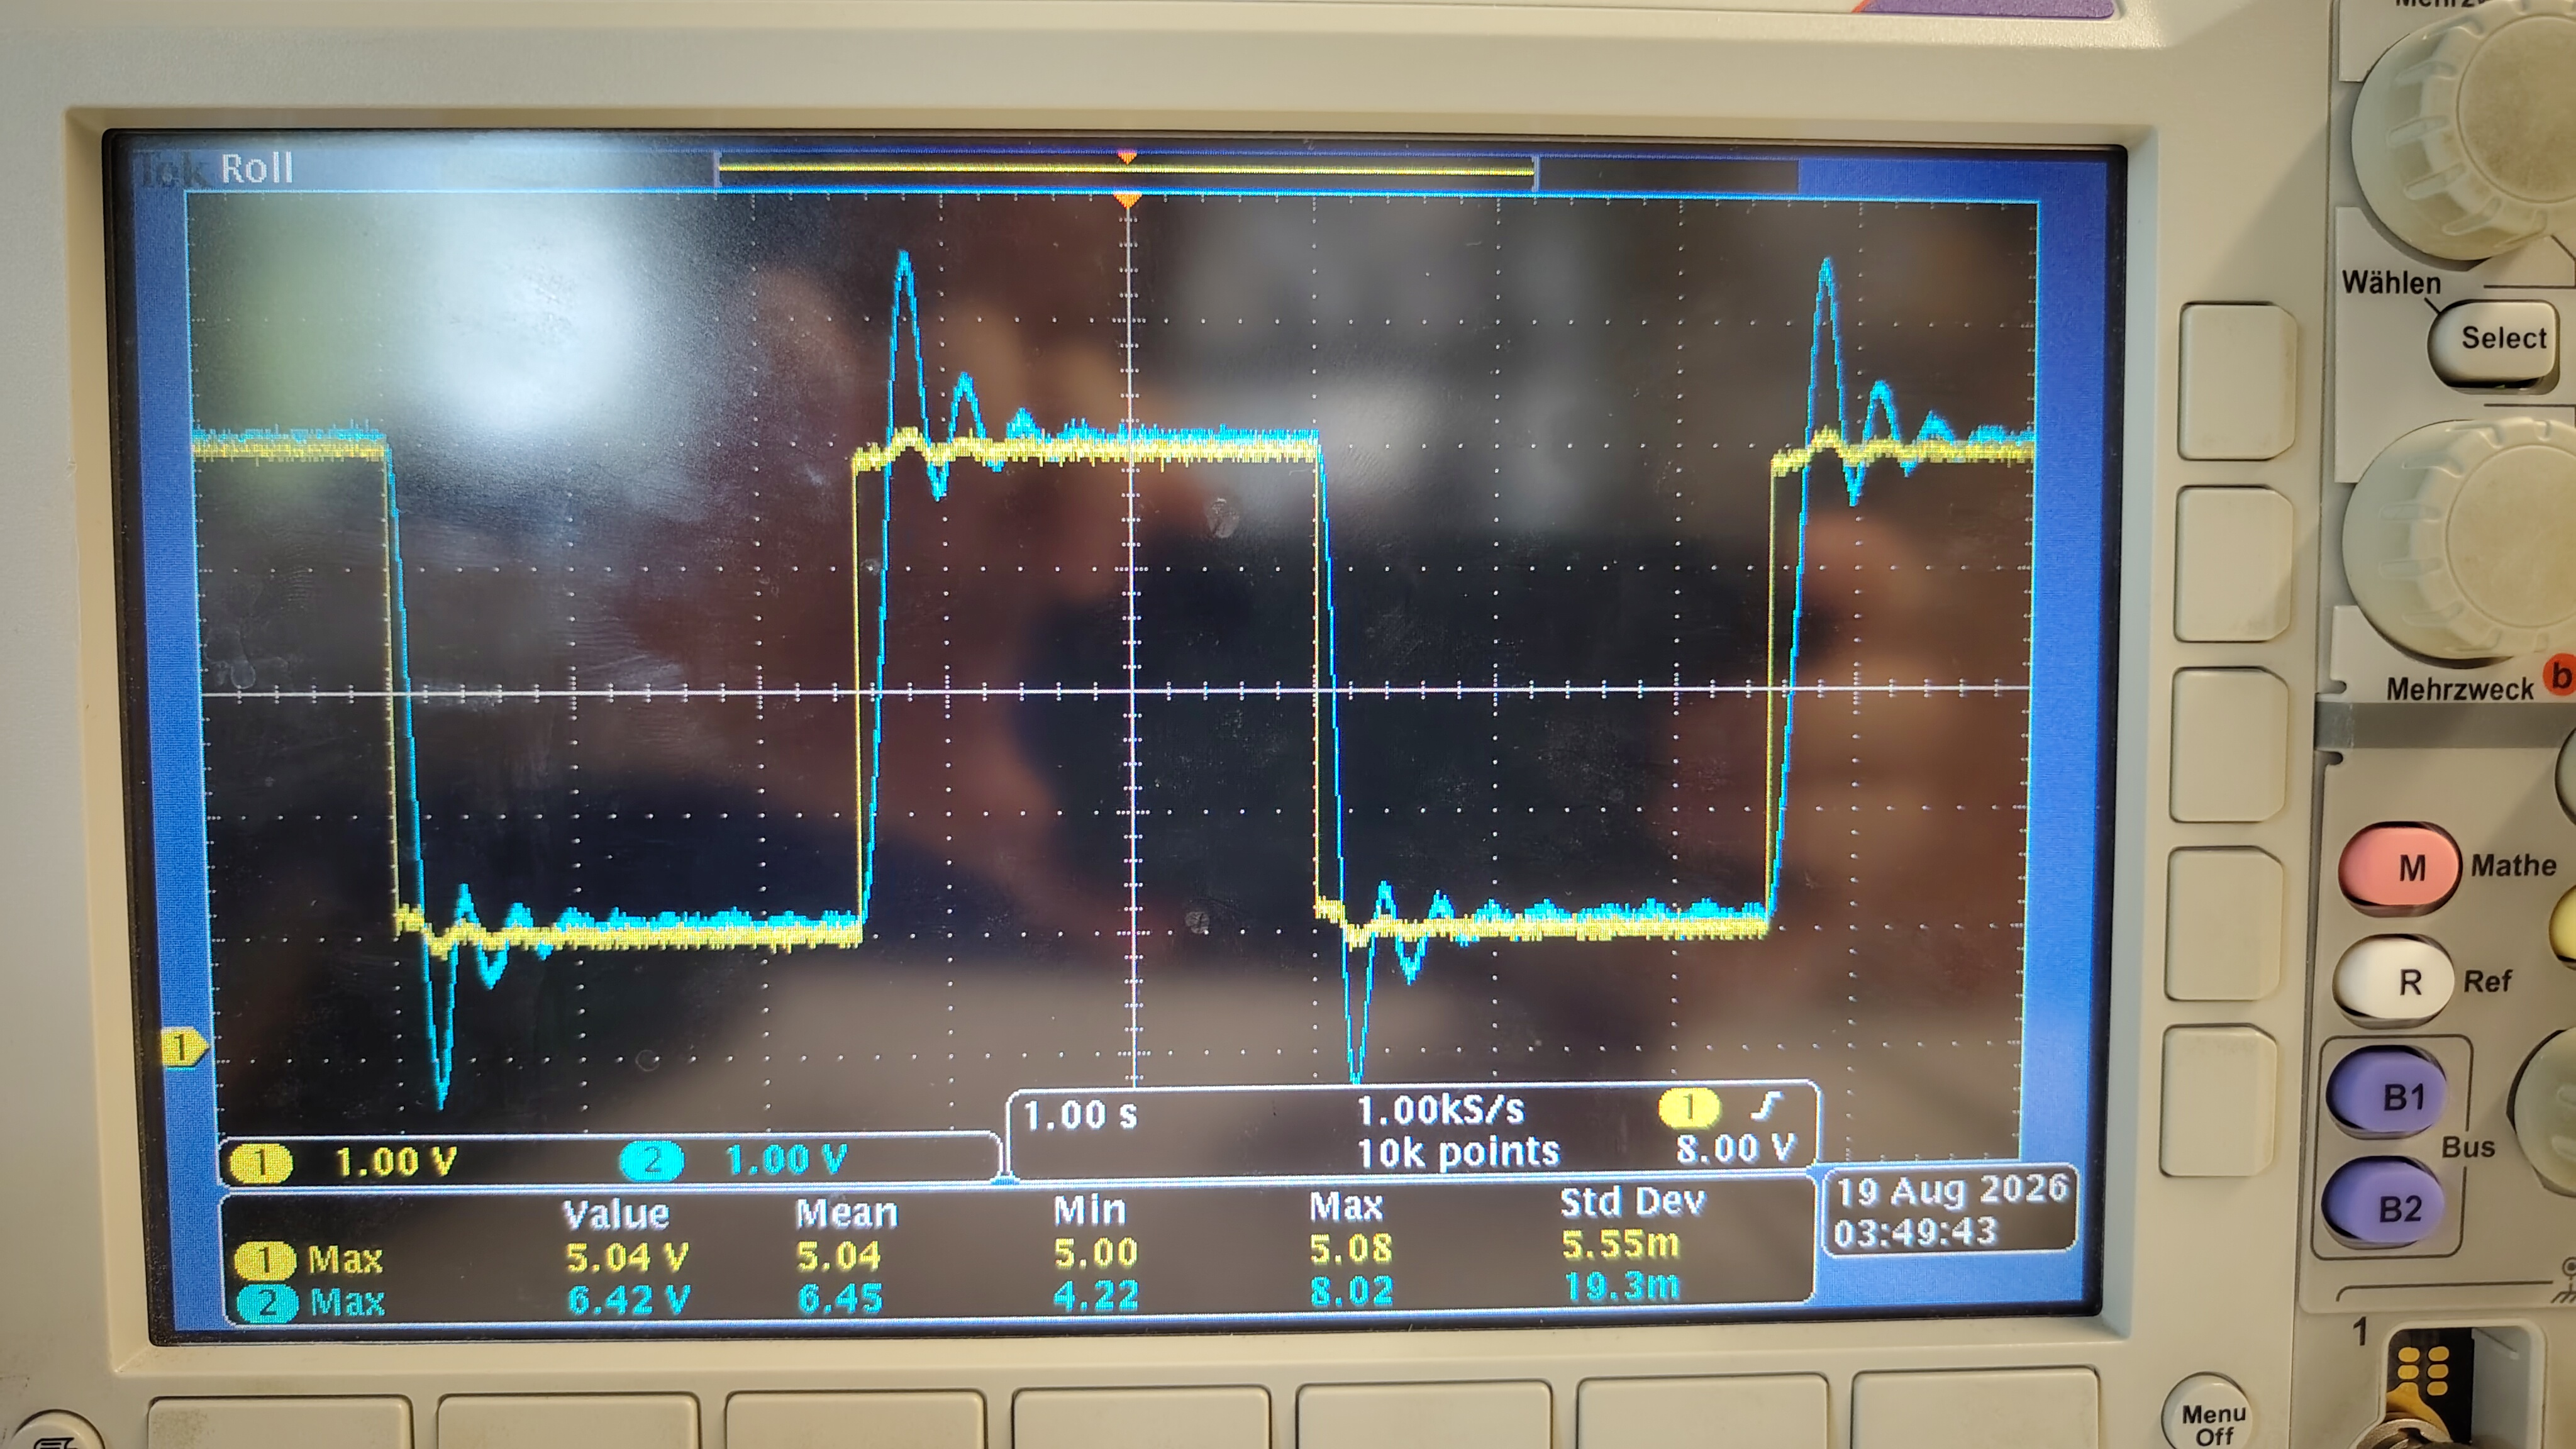
\includegraphics[width=\textwidth]{P_100_I_50}
    \caption{$K_p=100$ Skt, $K_I=50$ Skt}
    \label{fig:p=100_i=50}
    \end{subfigure}
    \hfill
    \begin{subfigure}[b]{0.48\textwidth}
    \centering
    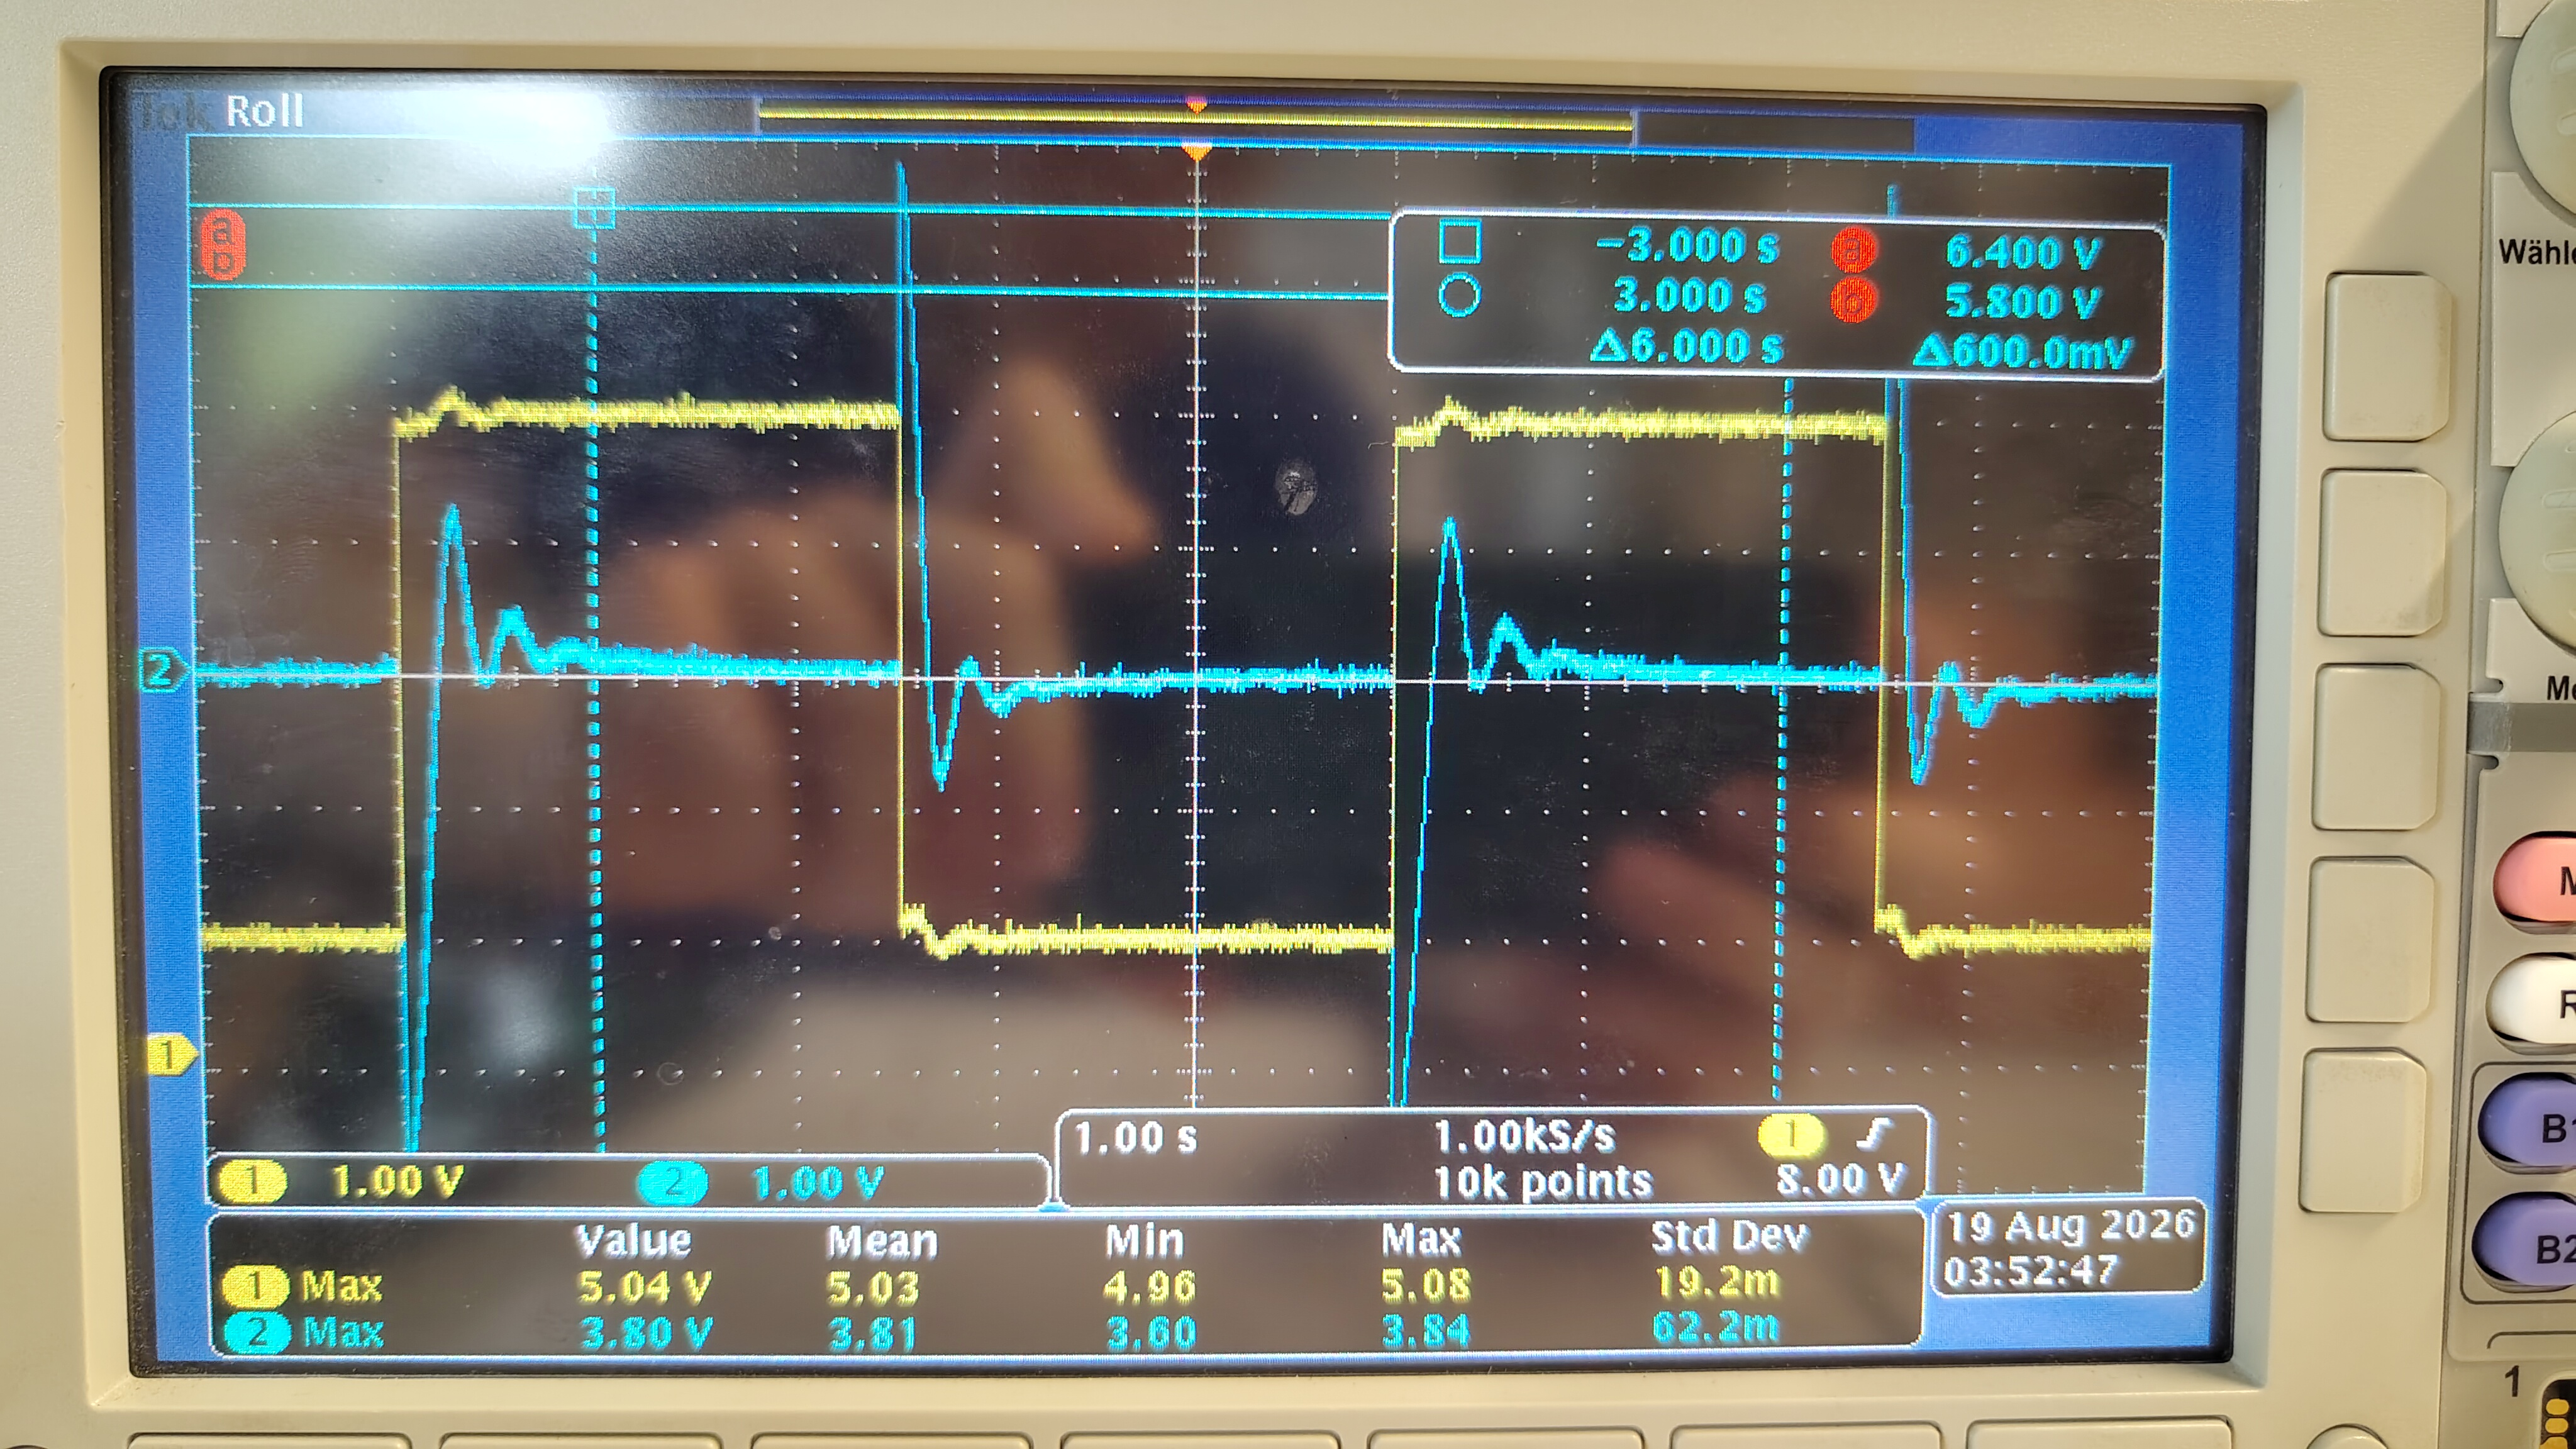
\includegraphics[width=\textwidth]{P_100_I_10_ist-soll}
    \caption{$K_p=100$ Skt, $K_I=10$ Skt, blau: Ist-Soll}
    \label{fig:p=100_i=50_ist-soll}
    \end{subfigure}
    \caption{PI-Regler mit unterschiedlichen $K_P$ und $K_I$ Kombinationen, in (f): Ist-Soll}
    \label{fig:PI-Regler}
\end{figure}
    \clearpage
    \begingroup
    \hypersetup{urlcolor=.,citecolor=citerullink}       % set linkcolour for bib to fontcolour
    \printbibliography[heading=bibintoc,title={Literaturquellen},filter={literature}]
    \printbibliography[heading=bibintoc,title={Abbildungsquellen},filter={figures}]
    \endgroup
    \hypersetup{urlcolor=blueurllink}                   % back to blue
    \clearpage
    \appendix
    \renewcommand{\thesubsection}{\thesection.\arabic{subsection}}

% ==============================================================================
% 1. EMITTERSCHALTUNG
% ==============================================================================
\section{Dimensionierungsberechnung}
\label{sec:Dimensionierung}
Anhand vorgegebener Parameter und den theoretischen Erläuterungen sowie Gleichungen im Skript\autocite{Skript_01} wurden die Größen der zu verwendenden Bauteile sowie die anschließend im Experiment zu messenden Größen berechnet. Die Widerstände und Kondensatoren wurden hierzu an die Normreihe E12 angepasst. Alle mit \enquote{Norm} indizierten Werte (also Spannungen, etc) wurden dann sukzessive mit den genormten Bauteilgrößen berechnet. 
Die Größen werden in diesem Format angegeben:
\begin{flalign*}
  \hspace*{1.5cm} X_i = f(x_i) &&&& = X_{\mathrm{Norm}}\text{[a.u.]} \quad (X_{\mathrm{theo}}\text{[a.u.]})
\end{flalign*}

\subsection{Emitterschaltung}
\subsubsection*{Gesetzte Parameter}
Randbedingungen (vom Aufbau vorgegebene Parameter):
\begin{itemize}
  \item Versorgungsspannung: $U_V = \qty{15}{\volt}$ (am Experiment eingestellt)
  \item Stromverstärkungsfaktor: $\beta \approx 400$ (\(\defeq h_{\mathrm{FE}}\) in \cite[58]{Skript_01}, Eigenschaft des Transistors BC457C)
  \item Basis-Emitter-Spannung: $U_{BE} \approx \qty{0.6}{\volt}$ (\(\defeq V_{\mathrm{BE}}(\mathrm{on})\) in \cite[58]{Skript_01}, Flussspannung der Silizium Diode des Transistors)
\end{itemize}
Gewünschte Parameter:
\begin{itemize}
  \item Kollektorstrom: $I_C = \qty{1}{\milli\ampere}$
  \item Spannungsverstärkung: $V_U = 20$
  \item Untere Grenzfrequenz: $f_{ug} = \qty{100}{\hertz}$
\end{itemize}

Berechnung des erforderlichen Basisstroms:
\begin{flalign*}
  &\hspace*{1.5cm} I_B = \frac{I_C}{\beta} &&&& = \qty{2.50}{\micro\ampere} \\
  \intertext{Dimensionierung des Kollektorwiderstandes $R_C$:}
  &\hspace*{1.5cm} R_C = \frac{U_V}{2 \cdot I_C \cdot \left(1 + \frac{1}{V_U}\right)} &&&& = \qty{6.80}{\kilo\ohm} \quad (\qty{7.14}{\kilo\ohm}) \\
  \intertext{Berechnung der Kollektorspannung $U_C$:}
  &\hspace*{1.5cm} U_C = R_C \cdot I_C &&&& = \qty{6.80}{\volt} \quad (\qty{7.14}{\volt}) \\
  \intertext{Dimensionierung des Emitterwiderstandes $R_E$:}
  &\hspace*{1.5cm} R_E = \frac{R_C}{V_U} &&&& = \qty{330.00}{\ohm} \quad (\qty{357.14}{\ohm}) \\
  \intertext{Berechnung der Emitterspannung $U_E$:}
  &\hspace*{1.5cm} U_E = R_E \cdot I_C &&&& = \qty{0.33}{\volt} \quad (\qty{0.36}{\volt}) \\
  \intertext{Berechnung der Kollektor-Emitter-Spannung $U_{CE}$ im Arbeitspunkt:}
  &\hspace*{1.5cm} U_{CE} = U_V - U_E - U_C &&&& = \qty{7.87}{\volt} \quad (\qty{7.50}{\volt}) \\
  \intertext{Berechnung der Spannung $U_{R2}$ am unteren Widerstand des Basisspannungsteilers:}
  &\hspace*{1.5cm} U_{R2} = U_{BE} + U_E &&&& = \qty{0.93}{\volt} \quad (\qty{0.96}{\volt}) \\
  \intertext{Dimensionierung des unteren Spannungsteilerwiderstandes $R_2$ ($I_{R_2} \geq 5 \cdot I_B$ nach Vorgabe):}
  &\hspace*{1.5cm} R_2 = \frac{U_{R2}}{5 \cdot I_B} &&&& = \qty{68.00}{\kilo\ohm} \quad (\qty{74.39}{\kilo\ohm}) \\
  \intertext{Dimensionierung des oberen Spannungsteilerwiderstandes $R_1$ ($I_{R_1} \geq 6 \cdot I_B$):}
  &\hspace*{1.5cm} R_1 = \frac{U_V - U_{R2}}{6 \cdot I_B} &&&& = \qty{820.00}{\kilo\ohm} \quad (\qty{937.99}{\kilo\ohm}) \\
  \intertext{Berechnung der Spannung $U_{R1}$ am oberen Widerstand des Basisspannungsteilers:}
  &\hspace*{1.5cm} U_{R1} = U_V - U_{R2} &&&& =\qty{14.07}{\volt} \quad (\qty{14.04}{\volt}) \\
  \intertext{Berechnung des effektiven Gesamteingangswiderstandes $R_{\text{EIN}}$ der gesamten Schaltung:}
  &\hspace*{1.5cm} R_{\text{EIN}} = \frac{1}{\frac{1}{R_1} + \frac{1}{R_2} + \frac{1}{\beta \cdot R_E}} &&&& = \qty{42.55}{\kilo\ohm} \quad (\qty{47.33}{\kilo\ohm}) \\
  \intertext{Bestimmung des effektiven Ausgangswiderstandes $R_{\text{AUS}}$ der gesamten Schaltung:}
  &\hspace*{1.5cm} R_{\text{AUS}} = R_C &&&& = \qty{6.80}{\kilo\ohm} \quad (\qty{7.14}{\kilo\ohm}) \\
  \intertext{Dimensionierung der Eingangskapazität $C_{\text{EIN}}$ für die untere Grenzfrequenz $f_{ug}$, anschließendes Verdreifachen aus Sicherheitsgründen:}
  &\hspace*{1.5cm} C_{\text{EIN}} = \frac{1}{2 \cdot \pi \cdot R_{\text{EIN}} \cdot f_{ug}} &&&& = \qty{100.00}{\nano\farad} \quad (\qty{33.63}{\nano\farad}) \\
  \intertext{Dimensionierung der Ausgangskapazität $C_{\text{AUS}}$ für die untere Grenzfrequenz $f_{ug}$ und Überdimensionierung aus Sicherheitsgründen:}
  &\hspace*{1.5cm} C_{\text{AUS}} = \frac{1}{2 \cdot \pi \cdot R_{\text{AUS}} \cdot f_{ug}} &&&& = \qty{1.00}{\micro\farad} \quad (\qty{222.82}{\nano\farad})\\
  \intertext{erneutes Berechnen der unteren Grenzfrequenz mit neu gewählter Kapazität:}
  &\hspace*{1.5cm} f_{ug}=(2\pi\cdot R_{\text{EIN}} \cdot C_{\text{EIN}})^{-1} &&&& =\qty{37.40}{\hertz}
\end{flalign*}

% ==============================================================================
% 2. KOLLEKTORSCHALTUNG
% ==============================================================================
\subsection{Kollektorschaltung}
\subsubsection*{Randbedingungen/gewünschte Parameter}
\begin{multicols}{2}
\begin{itemize}
  \item Versorgungsspannung: $U_V = \qty{15}{\volt}$
  \item Stromverstärkungsfaktor: $\beta = 400$
  \item Basis-Emitter-Spannung: $U_{BE} = \qty{0.6}{\volt}$
  \item Untere Grenzfrequenz: $f_{ug} = \qty{100}{\hertz}$
  \item Emitterstrom / Kollektorstrom: $I_E = I_C = \qty{15}{\milli\ampere}$  
\end{itemize}
\end{multicols}
Berechnung des erforderlichen Basisstroms:
\begin{flalign*}
  &\hspace*{1.5cm} I_B = \frac{I_C}{\beta} &&&& = \qty{37.50}{\micro\ampere} \\
  \intertext{Dimensionierung des Emitterwiderstandes $R_E$ für $U_V/2$ am Emitter:}
  &\hspace*{1.5cm} R_E = \frac{U_V}{2 \cdot I_C} &&&& = \qty{470.00}{\ohm} \quad (\qty{500.00}{\ohm}) \\
  \intertext{Berechnung der effektiven Emitterspannung $U_E$:}
  &\hspace*{1.5cm} U_E = R_E \cdot I_C &&&& = \qty{7.05}{\volt} \quad (\qty{7.50}{\volt}) \\
  \intertext{Berechnung der Basisspannung $U_{R2}$:}
  &\hspace*{1.5cm} U_{R2} = \frac{U_V}{2} + U_{BE} &&&& = \qty{8.10}{\volt} \\
  \intertext{Dimensionierung des unteren Spannungsteilerwiderstandes $R_2$:}
  &\hspace*{1.5cm} R_2 = \frac{U_{R2}}{5 \cdot I_B} &&&& = \qty{39.00}{\kilo\ohm} \quad (\qty{43.20}{\kilo\ohm}) \\
  \intertext{Dimensionierung des oberen Spannungsteilerwiderstandes $R_1$:}
  &\hspace*{1.5cm} R_1 = \frac{U_V - U_{R2}}{6 \cdot I_B} &&&& = \qty{27.00}{\kilo\ohm} \quad (\qty{30.67}{\kilo\ohm}) \\
  \intertext{Berechnung des effektiven Gesamteingangswiderstandes $R_{\text{EIN}}$ der gesamten Schaltung:}
  &\hspace*{1.5cm} R_{\text{EIN}} = \frac{1}{\frac{1}{R_1} + \frac{1}{R_2} + \frac{1}{\beta \cdot R_E}} &&&& = \qty{14.71}{\kilo\ohm} \quad (\qty{16.46}{\kilo\ohm}) \\
  \intertext{Bestimmung des effektiven Ausgangswiderstandes $R_{\text{AUS}}$ der gesamten Schaltung:}
  &\hspace*{1.5cm} R_{\text{AUS}} = R_E &&&& = \qty{470.00}{\ohm} \quad (\qty{500.00}{\ohm}) \\
  \intertext{Dimensionierung der Eingangskapazität $C_{\text{EIN}}$ und Überdimensionierung aus Sicherheitsgründen:}
  &\hspace*{1.5cm} C_{\text{EIN}} = \frac{1}{2 \cdot \pi \cdot R_{\text{EIN}} \cdot f_{ug}} &&&& = \qty{220.00}{\nano\farad} \quad (\qty{96.70}{\nano\farad}) \\
  \intertext{Dimensionierung der Ausgangskapazität $C_{\text{AUS}}$ für die untere Grenzfrequenz $f_{ug}$ und Überdimensionierung aus Sicherheitsgründen:}
  &\hspace*{1.5cm} C_{\text{AUS}} = \frac{1}{2 \cdot \pi \cdot R_{\text{AUS}} \cdot f_{ug}} &&&& = \qty{10.00}{\micro\farad} \quad (\qty{3.18}{\micro\farad})
  \intertext{erneutes Berechnen der unteren Grenzfrequenz mit neu gewählter Kapazität:}
  &\hspace*{1.5cm} f_{ug}=(2\pi\cdot R_{\text{EIN}}\cdot C_{\text{EIN}})^{-1}&&&&=\qty{49.10}{\hertz}
\end{flalign*}

% ==============================================================================
% 3. PID-REGLER
% ==============================================================================
\subsection{PID-Regler}
\subsubsection*{Gesetzte Parameter}
\begin{itemize}
  \item Widerstände: $R_2 = \qty{1.5}{\kilo\ohm}$, $R_5 = \qty{1}{\kilo\ohm}$, $R_7 = \qty{470}{\kilo\ohm}$, $R_8 = \qty{12}{\kilo\ohm}$, $R_{10} = \qty{100}{\kilo\ohm}$, $R_{17} = \qty{100}{\kilo\ohm}$, $R_{18} = \qty{2.2}{\kilo\ohm}$, $R_{23} = \qty{10}{\kilo\ohm}$, $R_{25} = \qty{10}{\kilo\ohm}$
  \item Kapazität D-Glied: $C_4 = \qty{220}{\nano\farad}$
  \item Grenzfrequenz / Verstärkung: $\omega_g = \qty{10}{\per\second}$, $V_{\min} = 1.15$
  \item Reglerkenngrößen: $K_{0,\min} = 1$, $K_{P,\min} = 1.5$, $K_{I,\min} = \qty{10}{\per\second}$, $K_{D,\min} = \qty{0.001}{\second}$
\end{itemize}

Dimensionierung der Tiefpasskapazität $C_6$ zur Istwertanpassung:
\begin{flalign*}
  &\hspace*{1.5cm} C_6 = \frac{1}{\omega_g \cdot R_{17}} &&&& = \qty{1.00}{\micro\farad} \\
  \intertext{Dimensionierung von $R_{19}$ für den nicht-invertierenden Verstärker:}
  &\hspace*{1.5cm} R_{19} = \frac{R_{18}}{V_{\min} - 1} &&&& = \qty{15.00}{\kilo\ohm} \quad (\qty{14.67}{\kilo\ohm}) \\
  \intertext{Symmetrische Widerstände des Subtrahierers:}
  &\hspace*{1.5cm} R_{21} = R_{22} = R_{24} = R_{23} &&&& = \qty{10.00}{\kilo\ohm} \\
  \intertext{Dimensionierung des Eingangswiderstandes $R_1$ für das P-Glied:}
  &\hspace*{1.5cm} R_1 = \frac{P_{1,\min} + R_2}{K_{P,\min}} &&&& = \qty{1.00}{\kilo\ohm} \\
  \intertext{Dimensionierung des Widerstandes $R_6$ für das I-Glied:}
  &\hspace*{1.5cm} R_6 = K_{0,\min} \cdot R_5 + P_{2,\min} &&&& = \qty{1.00}{\kilo\ohm} \\
  \intertext{Dimensionierung des Integrierkondensators $C_5$:}
  &\hspace*{1.5cm} C_5 = \frac{P_{2,\min} + R_6}{R_5 \cdot R_7 \cdot K_{I,\min}} &&&& = \qty{220.00}{\nano\farad} \quad (\qty{212.77}{\nano\farad}) \\
  \intertext{Dimensionierung des Eingangswiderstandes $R_4$ für das D-Glied:}
  &\hspace*{1.5cm} R_4 = \frac{K_{D,\min}}{C_4} &&&& = \qty{4.70}{\kilo\ohm} \quad (\qty{4.55}{\kilo\ohm}) \\
  \intertext{Symmetrie-Widerstände für Inverter-Stufen:}
  &\hspace*{1.5cm} V=-1=\frac{R_{26}}{R_{25}}\implies R_{26} = R_{25} &&&& = \qty{10.00}{\kilo\ohm} \\
  &\hspace*{1.5cm} V=-1=\frac{R_{9}}{R_{8}}\implies R_9 = R_8 &&&& = \qty{12.00}{\kilo\ohm} \\
  \intertext{Widerstände des Summierers / Addierers:}
  &\hspace*{1.5cm} U_s=\underbrace{\frac{R_{13}}{R_{10}}}_{=1}U_P+\underbrace{\frac{R_{13}}{R_{R_{11}}}}_{=100}U_I+\underbrace{\frac{R_{13}}{R_{12}}}_{=1}U_D\implies R_{12} = R_{13} = R_{10} &&&& = \qty{100.00}{\kilo\ohm}\\
  &\hspace*{1.5cm} \implies R_{11}=\frac{R_{13}}{100}&&&&=\qty{1.00}{\kilo\ohm}
\end{flalign*}   

\section{Bauteilergebnisse}
\sisetup{
  table-format = 6.2,           % Globales Zahlenformat (3 Vorkommastellen, 2 Nachkommastellen)
  table-number-alignment = center, % Alignment für S-Spalten (z. B. center, right)
  % Falls du \qty direkt in S-Spalten nutzt:
}
Hier werden noch einmal kurz übersichtlich nur bauteilspezifische Größen aufgelistet, also Widerstände und Kapazitäten der zu verlötenden Widerstände. Für die Kollektor- und Emitterschaltung wurden die Kapazitätswerte überdimensioniert und der passendste Normwert ausgewählt. Bei der PID-Schaltung ist keine sicherheitsmotivierte Anpassung der Kapazitätswerte notwendig.
\begin{table}[htbp]
  \centering
  \caption{Dimensionierung der Widerstände und Kapazitäten der Emitterschaltung}
  \begin{tabularx}{0.8\textwidth}{@{\hspace{0.5cm}} L  @{\extracolsep{\fill}} S @{\extracolsep{\fill}} S }
    \toprule
    \text{Bauteil} & {\text{theoretisch}} & {\text{Normreihe}} \\
    \midrule
    R_C \, [\unit{\kilo\ohm}]       & 7.14   & 6.80 \\
    R_E \, [\unit{\ohm}]            & 357.14 & 330.00 \\
    R_1 \, [\unit{\kilo\ohm}]       & 936.19 & 820.00 \\
    R_2 \, [\unit{\kilo\ohm}]       & 76.57  & 68.00 \\
    C_{\text{EIN}} \, [\unit{\nano\farad}] & 33.63  & 100.00 \\
    C_{\text{AUS}} \, [\unit{\nano\farad}] & 222.82 & 1000.00 \\
    \bottomrule
  \end{tabularx}
  \label{table:emitterschaltung}  
\end{table}

\begin{table}[htb]
  \centering
  \caption{Dimensionierung der Widerstände und Kapazitäten der Kollektorschaltung}
  \begin{tabularx}{0.8\textwidth}{@{\hspace{0.5cm}} L  @{\extracolsep{\fill}} S  @{\extracolsep{\fill}} S}
    \toprule
    \text{Bauteil} & {\text{theoretisch}} & {\text{Normreihe}} \\
    \midrule
    R_E \, [\unit{\ohm}]            & 500.00 & 470.00 \\
    R_1 \, [\unit{\kilo\ohm}]       & 30.67  & 27.00 \\
    R_2 \, [\unit{\kilo\ohm}]       & 43.20  & 39.00 \\
    C_{\text{EIN}} \, [\unit{\nano\farad}] & 96.70  & 220.00 \\
    C_{\text{AUS}} \, [\unit{\nano\farad}] & 3183.10 & 10000.00 \\
    \bottomrule
  \end{tabularx}
  \label{table:kollektorschaltung}  
\end{table}

\begin{table}[htb]
  \centering
  \caption{Dimensionierung der Widerstände und Kapazitäten der PID-Schaltung}
  \begin{tabularx}{0.8\textwidth}{@{\hspace{0.5cm}} L @{\extracolsep{\fill}} S @{\extracolsep{\fill}} S}
    \toprule
    \text{Bauteil} & {\text{theoretisch}} & {\text{Normreihe}} \\
    \midrule
    R_1 \, [\unit{\kilo\ohm}]       & 1.00   & 1.00 \\
    R_4 \, [\unit{\kilo\ohm}]       & 4.55   & 4.70 \\
    R_6 \, [\unit{\kilo\ohm}]       & 1.00   & 1.00 \\
    R_9 \, [\unit{\kilo\ohm}]       & 12.00  & 12.00 \\
    R_{11} \, [\unit{\kilo\ohm}]    & 1.00   & 1.00 \\
    R_{12}, R_{13} \, [\unit{\kilo\ohm}] & 100.00 & 100.00 \\
    R_{19} \, [\unit{\kilo\ohm}]    & 14.67  & 15.00 \\
    R_{21}, R_{22}, R_{24} \, [\unit{\kilo\ohm}] & 10.00 & 10.00 \\
    R_{26} \, [\unit{\kilo\ohm}]   & 10.00  & 10.00 \\
    C_5 \, [\unit{\nano\farad}]     & 212.77 & 220.00 \\
    C_6 \, [\unit{\nano\farad}]     & 1000.00 & 1000.00 \\
    \bottomrule
  \end{tabularx}
  \label{table:pid_schaltung}  
\end{table}

\section{Widerstandsnormreihe E12}
\label{sec:E12}
Nach Skript\autocite{Skript_01} sind \enquote{Widerstände [\dots] in internationalen Normreihen klassifiziert.} Die theoretisch berechneten Werte werden also an die zur Verfügung stehenden Normwerte angepasst, indem der Normwert mit der kleinsten Abweichung verwendet wurde. Es steht für Widerstände die Normreihe E12 zur Verfügung:
\[(\numlist{1.0;1.2;1.5;1.8;2.2;2.7;3.3;3.9;4.7;5.6;6.8;8.2})\cdot 10^{0}-10^{5}\;\unit{\ohm}\]

% \section{Code-Anhang}
% Bei den Funktionen habe ich teilweise Dinge von verschiedenen Altprotokollen zusammengesucht, und auf meine Bedürfnisse umgeschrieben. Die konkreten Berechnung sind dann eigenständig.
% \includepdf[pages=-]{../Code/241/241.pdf}
\end{document}